\documentclass[12pt]{myucthesis}
% This enables, e.g., clicking in Skim's PDF view (on OSX) to open the relevant
% source file in Vim
% For some reason, luaTeX doesn't seem to like it, doing command line now
% \synctex=1

% \nofiles
% The above command prevents latex from writing its auxiliary
% files. This is useful if you want to manually tweak them before you
% generate your final PDF. But it will break reference / bibliography
% resolution!

% This lets us load OpenType fonts from the system without any fuss. 
% It's already required by unicode-math, but I include it for reference.
\usepackage{fontspec}

% \usepackage{amsmath,amssymb}

% Note that if you use unicode-math, you need to do it after amsmath (and prehaps other
% ams things) Using unicode-math as recommended by the libertine package
% documentation

% This is one approach to doing maths in the context of libertine
% These are options that don't matter to this document!
% \usepackage[partial=upright,nabla=upright]{unicode-math}
% Note that none of the 4 styles available in unicode-math adhere to APA! french
% is closest / easiest, as only upright latin characters are wrong (they should
% be italicised, but they are not). Can use \mathit
\usepackage[math-style=french]{unicode-math}
% What can I say, I love the french
\frenchspacing

% microtype enables subtle typography improvements.
% Note that in XeTeX, expansion is disabled, and so some line breaks get screwed
% up (and you need to manually include hyphens or similar)
\usepackage{microtype}
% DJC - I'm doing all kinds of fussing around to get decent math type setting
% Oh fussiness! The below is an alternative way to use microtype (that didn’t
% work properly for me)
% \newfontfeature{Microtype}{protrusion=default;expansion=default;}

% This keeps things like `` and --- working
\defaultfontfeatures{Ligatures=TeX}
% NB: Numbers=OldStyle can only be used on the regular Pagella font
% The Microtype option for set*font is redundant with the microtype package
\setmainfont{TeX Gyre Pagella}
\setsansfont{TeX Gyre Heros}
\setmonofont{TeX Gyre Cursor}
\setmathfont{TG Pagella Math}

% Page layout. The fancyhdr package may complain about the need for a
% larger headheight, depending on how long chapter titles are; if left
% unspecified in the geometry setup, it defaults to 12pt. The
% "showframe" option causes the geometry package (version >= 5.0) to
% show a frame around the margins on every page, which is great for
% checking that you don't overflow anywhere.

% geometry driver auto detection may not work for XeLaTeX below
% \usepackage[letterpaper,includehead,margin=1in,headheight=15pt,showframe]{geometry}
\usepackage[letterpaper,includehead,margin=1in,headheight=15pt]{geometry}
\usepackage{fancyhdr}
\pagestyle{fancyplain}
\lhead[\fancyplain{\thepage}{\thepage}]{\fancyplain{}{\scshape\rightmark}}
\rhead[\fancyplain{}{\scshape\leftmark}]{\fancyplain{\thepage}{\thepage}}
\chead{}
\cfoot{}
\lfoot{}
\rfoot{}


% Bibliography stuff:
% DJC - I'm now using biblatex and bilatex-apa
% This is 1i18n overkill, including i18n of quotes
% Also - folks seem to think polyglossia is better now (only works in XeTeX, not
% LuaTeX)
\usepackage[american]{babel}
\usepackage{csquotes}

\usepackage[style=apa,backend=biber]{biblatex}

% More i18n overkill
\DeclareLanguageMapping{american}{american-apa}

\addbibresource{thesis.bib}
\addbibresource{fixed.bib}

% Other setup:

% Note: with BibLaTeX, you should load hyperref after the biblatex package.
\usepackage[pdfborder={0 0 0},pdfusetitle]{hyperref}
% This was the original hyperref inclusion with color
% \usepackage[colorlinks,urlcolor=blue,citecolor=blue,linkcolor=blue,pdfusetitle]{hyperref}
\usepackage{pdflscape} % allows landscape-oriented figures with PDF page rotation
\usepackage{graphicx}

% It strikes me as not worth checking into this given its age
% \usepackage{mydeluxetable} % deluxetable customized to play well with ucthesis

% DJC - my extra packages here
% This is where warnings about the caption package come from
\usepackage{subfig,multirow,hologo,underscore}
% Make it easier to print complicated tables
\usepackage{longtable,siunitx,tabu}
% This might be useful for simpler tables. For text heavy tables with
% Excel-style CSV, tex-based solutions are going to choke!
% \usepackage{pgfplotstable}
% Mostly just to supress a warning
% \pgfplotsset{compat=1.8}
% \pgfplotstableset{sci zerofill}%,col sep=comma}

% pgfplotstable recommends
% This will allow some of the nicer layout options for number alignment, etc.
% \usepackage{array}

% Better spacing and rules (lines, not laws)
\usepackage{booktabs}

\usepackage{pdfpages}

% May also need to use this if we decide to have some huge tables:
% But make sure we load things in the right order!
% \usepackage{longtable}

\begin{document}
\ssp % single spacing
\hypersetup{pageanchor=false}
\title{Climate Change and Conceptual Change}
\author{David J. Clark} % must match BearFacts!
\degreesemester{Fall}
\degreeyear{2013}
\degree{Doctor of Philosophy}
\numberofmembers{4}
\chair{Professor Michael A. Ranney}
\chairb{Professor Richard B. Ivry}
\othermembers{
Professor Sonia Bishop \\
Professor John Canny
}
\field{Psychology}
\campus{Berkeley}

\maketitle
\copyrightpage

\begin{abstract}
My work is awesome. Give me a Ph.D.
\end{abstract}

% DJC: another hyperref config
\hypersetup{pageanchor=true}
\begin{frontmatter}

\begin{dedication}
\null\vfil
{\large
\begin{center}
With love and respect for all that is good—in particular the unwavering
support of my grandma (even if she doesn't fully accept climate change).
\end{center}}
\null\vfil
\end{dedication}

\tableofcontents
\listoffigures % optional
\listoftables % optional

% If using code.sty, can also add:
%% \listofcodes
%% \addcontentsline{toc}{chapter}{List of Code Examples}

\begin{acknowledgements}
Thanks for all the help!

% Shout out to Larry Goldfarb.
% Feel free to modify or remove this acknowledgment:
This dissertation was based on the
\href{https://github.com/pkgw/ucastrothesis}{\textsf{ucastrothesis}}
% DJC non-hyperref alternative with plain textsf
% \textsf{ucastrothesis}
template. It was typeset with \hologo{LuaLaTeX} using the Pagella and Heros
fonts from the \TeX\ Gyre project.

\end{acknowledgements}
\end{frontmatter}

% \chapter{Introduction}
\label{c.intro}

% \epigraph{Let us, then, omit the conjectures of men who know not what they say,
%     when they speak of the nature and origin of the human race... They are
%     deceived, too, by those highly mendacious documents which profess to give
%     the history of many thousand years, though, reckoning by the sacred
%     writings, we find that not 6000 years have yet passed.}{St. Augustine, c.
%     397 CE}

Abstract goes here?

\section{The problem}

% Make this more of a lead-in to the rtmd, NDI and dual-system learning

Various human efforts, over the course of history, have drastically improved the
comprehensibility of our world. Along with this, the scope of our power to alter
our world has increased dramatically. Unfortunately, these alterations are not
always for the better, as is the case with global climate change. There is broad
agreement that anthropogenic (human caused) climate change is currently and will
continue to have negative consequences on both human and other forms of life on
our planet (for example, about 97\% of publishing climate scientists hold this
view). Certainly, some may say, the planet will endure. But, it seems wise
to proceed with some concern towards ensuring the survival of those organisms
and species we hold most dear.

While humans continue to increase our understanding of the world, issues like
climate change appear to be a bit beyond what is readily comprehended by
non-specialists. In particular, there seems to be a trouble with the
comprehension and acceptance of climate change in America. While much of the
developed world accepts anthropogenic climate change as a reality, as of January
2010 only 57\% of individuals surveyed in the United States think global warming
is happening at all. When asked to assume that global warming \emph{is}
happening, only 47\% of the same group of respondants indicated that they
thought it was ``caused mostly by human activities'' \cite<Q47 and Q50
in>{leiserowitz_climate_2010}.  Presumably, the number of Americans accepting
anthropogenic climate change is somewhat less than this figure. Thus, if we want
to do something about this issue in the context of a democratic society, the
first step is getting a reasonable majority of people to accept that there at
least \emph{may} be a problem \cite{prochaska_toward_1986}.  
% Note - Canny thinks the TTM cited here is not terribly relevant
Thus, the overarching question, ``How can ideas from cognitive science help us
improve climate change education?''

Certainly, the scope of climate change cognition is far too broad for a research
project of only a few semesters. As such, I will focus on a handful of issues
that are of interest from the point of view of a cognitive theory of learning.
Simultaneously, we maintain an educational point of view that entails a focus on
variables that we might control. I assume a pragmatic sense of ``poor'' and
``good'' cognition regarding climate change and related conceptual domains. The
goal will be to obtain an understanding that allows us to shift individuals from
the former to the latter. Roughly speaking, ``good'' cognition would allow
people to reason more accurately and be more robust to the problematic
arguments they are likely to encounter in our current political landscape.
Specific features of such cognition might include:

\begin{enumerate}
\item Reasoning with \emph{evidence}. In particular, the use of specific,
quantitative information (as discussed in section~\ref{sec:ndi} below).
\item Fluency with models used to explain and predict climate change.
\item Skeptical evaluation of evidence offered by others.
\item Ability to connect one's personal values and beliefs to policy
preferences.
\end{enumerate}

In an ideal world, the structure of this thesis would harken back to early
psychophysical research. There are a number of factors that we are certain will
induce surprise, acceptance of novel ideas and other forms of learning. A
lovely question could take the form of ``How many units of surprise yield so and
so units of attitudinal shift?'' or ``When matched for identical amounts of
cognition, what is the relative effect of numerically-grounded evidence vs.\
emotionally charged evidence?'' As is plain to see, such precision is well
beyond the current state of the art. Thus, I will focus primarily on categorical
differences between educational interventions and participants memories and
explanations. Below, I lay out a number of issues that figure heavily into the
selection of these categories.

\section{Reinforced Theistic Manifest Destiny theory}

%% Problematically, Al Gore also talks a lot about melting ice - arguing against
%% the bulk of our pro-GW items!

\citeA{ranney_why_inpress} observe that in addition to America's disparity
with peer nations in accepting global warming, Americans are also appreciably
lower in their acceptance of Darwinian evolution. Indeed, the United States
ranks 33rd of 34 peer nations in acceptance of evolution, putting us
squarely between Cypress and Turkey. The ``received view'' is that Americans are
particularly fundamentalist in their acceptance of biblical creation\footnote{I
will focus primarily on the Christian faith, as it is the dominant religion in
the U.S.\ and peer nations of interest. 84\% of Americans practice some form of
Christianity, with Judaism and Islam as the second and third most common at
1.9\% and 1.6\% respectively \cite{wolfram_alpha_faith}.}, 
necessitating the rejection of evolutionary ideas. But, this notion fails to
address the similar pattern observed with acceptance of climate change. In
addition, many of the afore-mentioned peer nations also exhibit high adherence
to Christian faiths.  Likewise, it is not clear that America is sufficiently
more fundamentalist than peer nations to explain all the important variance in
our acceptance of these ideas. 

\begin{figure}[h]
\centering
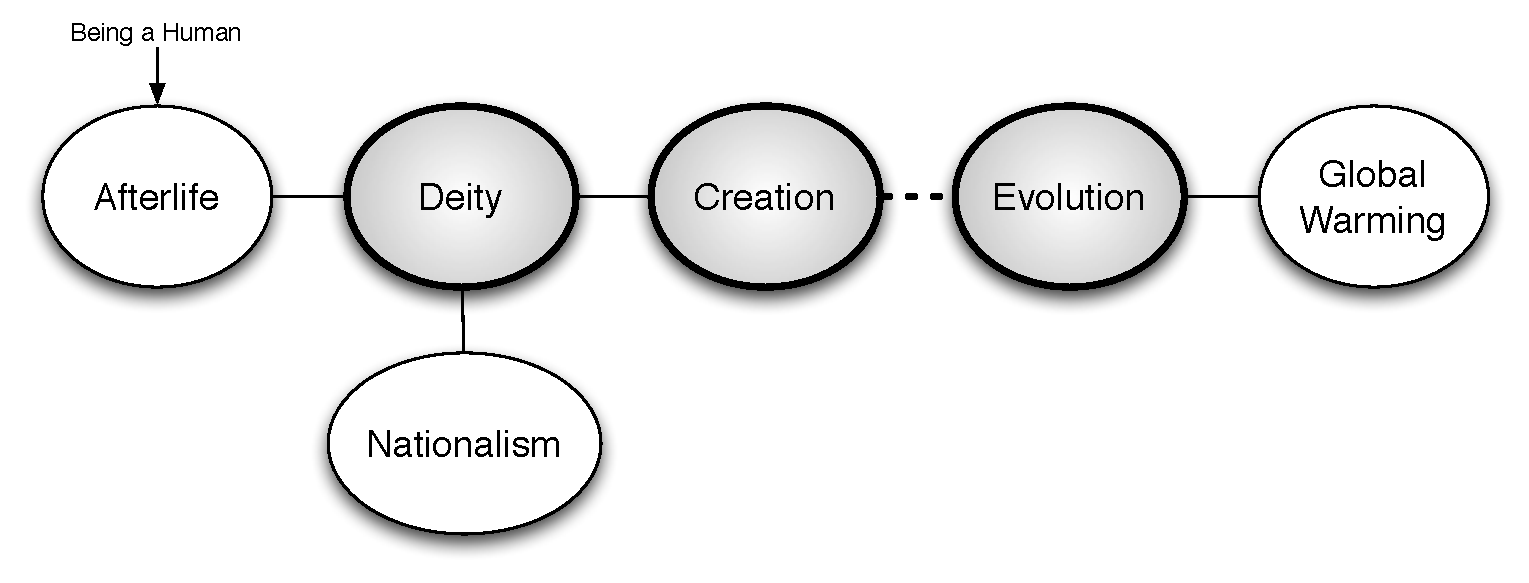
\includegraphics[width=\textwidth]{rtmd.pdf}
\caption{Ranney's RTMD model. The ``received view'' is emphasized, with
a negative relationship between belief in creation and acceptance of evolution
represented by the dashed line. Solid lines express positive relationships
between these and a network of related attitudes. A causal point of entry is
expressed for ``being a human,'' fearing death and thus, desiring an afterlife.}
\label{fig:rtmd} 
\end{figure}

The central insight of \citeA{ranney_accepting_2011} is that what sets the
United States apart from the rest of the world is the relative success it has
experienced over the previous century, called by some ``The American Century.''
Our war efforts have been (or at least seem) enormously successful, our economy
is far larger than any other economy in the world, we are successful in the
Olympics and so on. This leads to a
feeling that ``God is on our side,'' or in other words, it reinforces notions of
manifest destiny via quasi-religious sentiment.


Another general problem identified within RTMD is the fact that individuals
often reject scientific ideas when they are in conflict with their other
attitudes and beliefs. It's as if we are endowed with something of a conceptual
immune system, % Maybe elaborate more in thesis?
comprising religious and nationalistic beliefs in some, and more
scientifically grounded beliefs in others.  But note, there is a sharp distinction between
the kinds of ``emotional responses'' that might be experienced between climate
change and evolution. Specifically, climate change is something that
involves the ethical status of actions that we do every day, both individually
and as a society. Evolution, on the other hand, tends to incohere with
personally held religious beliefs, most directly divine creation, but then by
extension, deity and afterlife.

As an interesting side-note, both evolution and climate science require vastly
larger views of time as compared to many other sciences. The longest sample of
atmospheric greenhouse gasses and global temperature goes back an impressive
800,000 years.  Impressive, that is, until you consider that most major phyla
emerged around 530 million years ago (and have thus been influencing the climate
since that time).

% An interesting point of comparison would be Plate Tectonics (which apparently
% is also quite controversial in the south

RTMD doesn't disagree with other explanations, such as an analysis of
individuals into democrats and republicans. Rather, it provides a more specific
set of proximal relationships between concepts. According to the theory, for
example, acceptance of evolution should have \emph{more} predictive value for
one's global warming acceptance as compared to, say, acceptance of a deity.
Additionally, these relationships may predict related changes we might see as we
modulate individual's attitudes.


% Perhaps mention the inclusion of notions of consumerism?

\section{Reasoning with Numbers \label{sec:ndi}}

% It would probably make sense to highlight a more social psych citation here,
% as it would be more germane to climate change. Perhaps even one of the more
% recent climate change polarization articles?

NDI procedures \cite<introduced by>{ranney_numerically_2001_fixed} provide an
approach to changing conceptions, attitudes and even behaviors with quite
minimalist interventions (e.g., providing estimators with a single, critical,
highly germane, feedback statistic, \citeNP<cf.>{rinne_estimation_2006}).  The
education and social psychology literature provide multiple examples of failures
to elicit conceptual change. For example, \citeA{chi_commonsense_2005} describes
an intervention in which only 1 in 100 eighth-graders were able to shift to a
correct conceptual model of diffusion. Similar examples are available in a
variety of literatures \cite<cf.>{disessa_what_1998, lord_biased_1979}.
Certainly, the are marked differences between the above mentioned approaches to
conceptual change. For the purposes of the current effort, we will focus our
attention on those approaches that have been successful (namely, NDI and related
approaches).

One of the elements of the NDI program, The EPIC procedure, represents an
intervention that is relatively compact and well specified. More importantly,
EPIC has been shown to induce long-lasting conceptual change
\cite<e.g.,>{ranney_designing_2008}, as evidenced by increased accuracy on estimations
up to 12 weeks later \cite{munnich_longevities_2005}.  In the EPIC procedure,
participants engage with real-world numerical facts that bear on a societal
issue, such as abortion, criminal justice, the environment, etc.
\cite<e.g.,>{garcia_de_osuna_qualitative_2004_fixed,munnich_policy_2003_fixed}.  
People often poorly
estimate these quantities, such that the true values are surprising to many
individuals, and experimental research on NDI has provided the basis for
successful classroom curricula for both high school students and graduate
students in journalism
\cite{munnich_numerically-driven_2004,ranney_designing_2008}.  During the EPIC
procedure, participants

\begin{enumerate}
\item Provide an \textbf{Estimate} for each policy-relevant item,
\item State what they would \textbf{Prefer} each quantity to be, 
\item Receive actual quantities as feedback to \textbf{Incorporate} (as new
“Information”), and 
\item Indicate whether their preferences have \textbf{Changed} upon receiving feedback.
\end{enumerate}

Work that I'll describe below has examined the cognitive components of a simpler
Estimate-Inform procedure. Moving forwards, expanding into an exploration of
Preference allows for a clear point of connection with the attitudes treated by
the RTMD theory.

\section{Conceptual and ``less conceptual'' cognition\label{sec:two}}

In its limit, the conceptual domain is the space of cognitive processes where
everything is connected to everything. Strong examples would include Whorfian
theories in which language constrains visual perception
\cite{boroditsky_does_2001}, or the notion of embodied cognition claims in which
our emotional preferences for spatially arranged items may be guided by our
fluency with our own right or left sides \cite{casasanto_embodiment_2009}. A
more prosaic example illustrating the difference between more and less conceptual
processing is provided in \citeA{clark_assembling_2003}, in which learning with
pre-existing knowledge (specifically, encoding known words vs. plausible
pseudo-words) lowered demands on prefrontal and parietal working memory
structures.

Our mind is also endowed with a number of special-purpose, relatively stable,
fast, local (encapsulated) or ``hard-wired'' capacities. The ``motor
system''\footnote{There may be more than one motor system, but at least one of
them should serve to illustrate this point.} is an excellent example of this.
Conceptually, our motor experience is simple---we desire an object and simply
reach for it. Under the hood, an enormous number of degrees of freedom are
resolved, satisfying multiple complex constraints all without our awareness.
\citeA{clark_multiple_2010} construct a set of features that roughly describe
the nature of cognitive processing in more or less conceptual modes. I adapt the
table given there for Table~\ref{table:multiple}.  Depending on the needs of a
given behavior, learning (or performance) might be better handled by cognition
of one sort or the other. These criteria echo what is discussed in the decision
making literature \cite{kahneman_perspective_2003}.

\begin{table}
\begin{tabular}{p{0.5\textwidth}p{0.5\textwidth}}
\textbf{More conceptual} & \textbf{Less conceptual} \\ \hline \hline

Large amount of learning per trial that saturates quickly (high gain) &
Small, incremental amount of learning per trial (low gain) \\
\hline

Requires extra time, cognitive resources for processing &
Learns automatically without effort \\
\hline

Required for contextual learning &
Unimodal or modular learning \\
\hline

Accessible to awareness and conscious intention &
Impenetrable to awareness, operates independent of conscious strategies \\
\hline

Consolidation processes are enhanced during sleep &
Consolidates off-line with the simple passage of time \\
\hline

Ready transfer to related tasks &
Task-specific and inflexible \\
\hline

Rational and recollective &
Emotional and intuitive \\
\hline
\end{tabular}
\caption{Features of more or less conceptual processing. Adapted (liberally) from
\protect \citeA{clark_multiple_2010}} 
% Consider referencing Sloman's 2-systems2-systems here?
\label{table:multiple}
\end{table}

\subsection{Relating to RTMD}

Given these notions, we can revisit the RTMD theory and suggest that perhaps the
relationships in that theory have a less fully conceptual flavor.  That is, I
suspect individuals don't explicitly consider, say, their feelings of national
pride when cognizing about evolution.  This may be similar to a subjective
experience we've likely all had. We can learn lots of great well-reasoned things
about someone we don't like or accept, and yet we may come to like or accept
them only slowly (or not at all). It's not a completely rational process!

So, interventions that operate more on non-conceptual aspects of, say,
nationalism (i.e., via emotionally charged items) may enhance the effect of
these relationships (i.e., increase correlations between them, or cause shifts in
related attitudes) as compared to shifts elicited by more objective items (such
as a mechanistic explanation of climate change).  On the other hand, it may be
that ideas don't support or detract from one another unless they are both
consciously held in memory at the same time. If this is the case, bringing these
relationships to mind may strengthen RTMD related effects.
% Maybe read / cite Hoadley, et al. (1994)?

\subsection{Relating to NDI}

A fundamental question in cognition concerns the nature of what is learned. Some
well-established psychological learning and memory models
\cite{nadel_memory_1997} might predict that changes in estimation accuracy must
ultimately be mediated by the consolidation of episodic memory. In this case, we
would expect participants' reports of explicit memory for feedback (the “I” in
EPIC) to correlate well with improvements in estimation accuracy at subsequent
testing.  This would clearly be learning of a conceptual type.

Recent evidence suggests, however, that pre-existing conceptual structures can
be re-modeled in a highly efficient manner that may not rely as heavily on the
brain structures implicated in episodic memory formation
\cite{tse_schemas_2007,clark_assembling_2003}. In this case, we might expect
increases in estimation accuracy even when participants report no memory
whatsoever for the quantity provided as feedback---particularly if participants
had pre-existing knowledge to support such learning.

Evidence of pre-existing knowledge is indicated by surprise upon receiving
feedback, which implies an incorrect prior expectation regarding the true value.
However, subsequent learning that correlates with surprise might also be
explained by an account involving the emotional impact of the information
\cite{munnich_surprise_2007,thagard_hot_2006}.  Therefore, it is important to
assess not only surprise, but also whether the surprise had an emotional (i.e.,
less conceptual) character. It may be the case that surprise mediates improved
episodic memory. Alternatively, surprise and the existence of prior knowledge
may operate partly or wholly in parallel---mediating direct changes in semantic
memory.

Most generally, learning may be driven by the actual experience of surprise
\cite<e.g.,>{munnich_longevities_2005}.  In addition, improvements in estimation could be
driven by a direct (potentially approximate) episodic memory of feedback. Thus,
it seems useful to query participants' surprise, and whether it is of a more
emotional or conceptual sort. In addition, we can probe participants memory in
an attempt to assess conscious recollective ability. In the end, these processes
are certainly overlapping, but it may be possible to differentially drive some
aspects of learning and not others, etc.

\section{Summary}

There is a clear need for the development of educational interventions targeting
climate change acceptance and attitudes. Above, we have seen that there is some
indication that compact, evidence-based interventions may provide notable,
durable shifts in policy-relevant attitudes. In the chapters that follow, we
will more closely examine a set of experiments regarding these sorts of
approaches to climate change cognition, some completed and some proposed. These
experiments will illuminate some aspects of the psychological processing of such
interventions that appear central to understanding how a successful intervention
would work.

\section*{Acknowledgments}

Probably won't do acknowledgements in the intro, but this is a good placeholder.

%% Put a summary here?

% \section{Questions}
% 
% To recapitulate, I have laid out a number of categorical distinctions above.
% 
% \begin{enumerate}
% \item There is clear evidence that attitudes and beliefs treated by the RTMD theory
% are predictive of one another. This may be largely a cultural or societal
% artefact, in which case learning would be relatively confined within a
% construct. Or, these relationships may reflect the representational structure of
% these ideas in our minds, in which case we might expect a change in one part of
% that network to have effects elsewhere.
% \item Evidence may be objective and concrete (i.e., it may seem very
% \emph{factual}), or it may seem partisan and/or poorly defined. This feature of
% an argument may have differential effects on how much people are moved upon
% hearing the argument, and the retention of any such changes (or even gradual
% increase, as in the classic ``hypermnesia'' paradigm).
% \item There is strong evidence that cognition may occur in relatively isolated,
% automatic systems, or alternatively in a more integrated or conceptual fashion.
% We can seek to characterize what kind of process occurs during a given learning
% or production (memory or explanation) episode. Given this characterization, we
% can again observe the magnitude and timecourse of any changes that are elicited.
% \end{enumerate}
% 
% I will evaluate the following hypotheses.
% 
% \begin{enumerate}
% \item Increased knowledge and understanding will yield greater acceptance of
% climate change (and similarly with evolution).
% \item Emotional engagement will play a role in climate change acceptance or
% rejection, as well as enhancing learning.
% \item Based on the relative success of NDI interventions, I expect that
% numerically-grounded or mechanistic arguments will result
% in more durable shifts, both against the passage of time, and against
% interference or agnotology.
% \item Alternatively, methods of persuasion that appeal to emotion, non-quantitative
% depictions of negative consequences and ethical arguments may have larger
% immediate effects.
% \item Emotional responses (like emotional surprise) will trigger larger shifts
% in attitudes, or increase the likelihood of change in attitudes and learning in
% general.
% \item No single point of entry will be necessary - changing behavior, appeal to
% emotions or provision of rational argument should all be sufficient to have some
% effect on their own.
% \item Multiple methods of engagement in parallel should interact to yield
% greater shifts / learning than the sum of those methods individual effects.
% \item Other attitudes (as in RTMD) will differentially enhance or dampen changes in
% climate change cognition.
% \end{enumerate}
% 
% \section{Some notes on graphical models}
% 
% Throughout this document, I'll use graphical models to supplement tables and
% textual descriptions.
% 
% TODO: Write more about this here!

\graphicspath{{mechanism/}}

\chapter{Teaching the Mechanism of the Greenhouse Effect}
\label{chap:mechanism}

As described above, American's lag much of the world regarding acceptance of
anthropogenic climate change. Informally, Michael Ranney,
then other members of our group started questioning whether people were able to
mechanistically explain how human activities cause an increase in global mean
temperature.  Almost no one could provide a satisfactory explanation, including
us! Prof. Ranney, Lloyd Goldwasser, and Daniel Reinholz (along with input from
myself and Ron Cohen) proceeded to develop a short \~400-word description of the
mechanism. This text is reproduced in full in Appendix~\ref{app:400words}.
Before reading the text yourself, I would encourage you to spend 10 minutes
describing \emph{your} understanding either aloud or on paper.\footnote{If you
personally doubt the veracity of anthropogenic climate change, then you may
modify the exercise to describing the mechanism of the greenhouse effect, first
described by Nobel laureate XXX Ahreneous (Sp?) in \citeyear{Ahreneous} (and
accepted as fact since that time!).}

Given that our informal investigations implied that almost no-one knew the basic
concepts described in our 400 words, we initiated the line of research described
below. In these experiments, we sought to formally ask:

\begin{enumerate}
\item Is this lack of understanding for the mechanism of global climate change
    as pervasive as it seemed to be?
\item Does instruction regarding the mechanism of global climate change increase
    individuals' acceptance of the reality of anthropogenic climate change?
\end{enumerate}
Along the way, we additionally considered related aspects of learners’
experiences (the details of which are described below).

The history of educational research would imply that it’s quite difficult to arrive
at definitive answers to big policy qeustions. For example, phonics vs.
whole-word reading has been debated at least since the dawn of the Common Era,
as discussed in \textcite{history-reading-instruction}. Below, however, I report
on a series of experiments that argue strongly (if not definitively!) that
instruction regarding the pysical mechanism of the greenhouse effect appears to
have some positive effect on public acceptance of anthropogenic climate change.
As discussed above, such public acceptance seems central to any truly democratic
approach to the problem of climate change.

\section{Classroom interventions at UC and UT}
\label{sec:mech-classroom}

This experiment was a fairly thick observation of individuals' beliefs,
attitudes and knowledge. We sought to understand how a relatively brief 400-word
mechanistic explanation might affect these measures, as well as how this might
be modulated by prior commitment to one's own explanations and stated attitudes.
The general flow of the experiment is given in Figure~\ref{fig:mech-flow}.

\begin{figure}[h]
    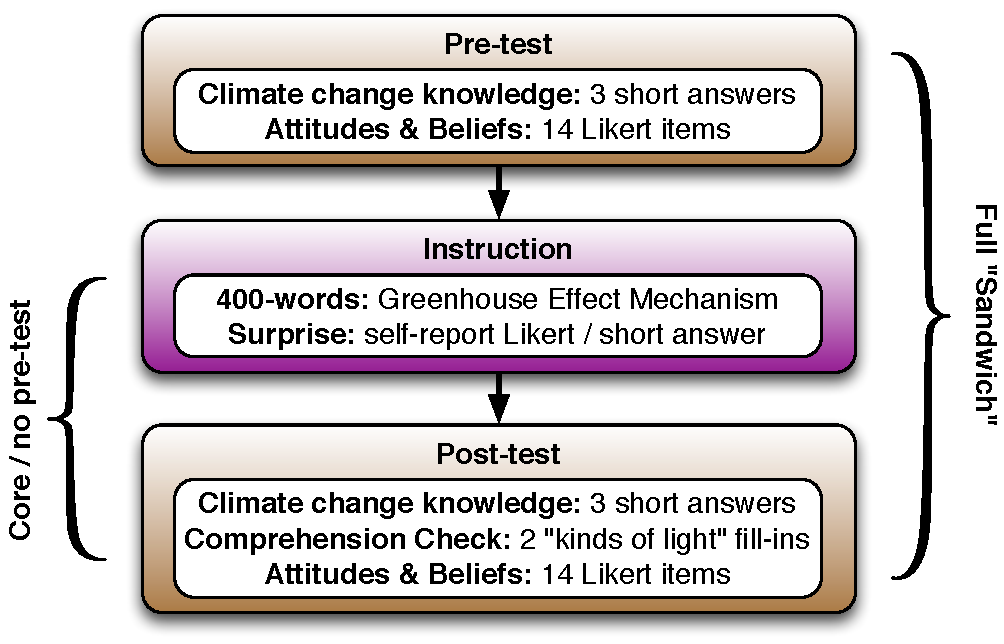
\includegraphics[width=6.5in]{mech-survey-flow1.pdf}
    \caption{An overview of experimental flow for
        Section~\ref{sec:mech-classroom}. Flow for other experiments in
        Chapter~\ref{chap:mechanism} was similar. The analogy to a sandwich
        takes the knowledge and attitutde tests to be slices of bread, and the
        educational intervention itself is the “jam.”}
    \label{fig:mech-flow}
\end{figure}

The primary goal here was a proof of concept. By assessing university
students---some of our nation’s most highly educated citizens---we provide a
strong test of our belief that most Americans are ignorant of the mechanism of
global climate change. An addition concern was that for maximal power, it is
preferable to sample na\"ive beliefs prior to the intervention. In such a
design, we are able to use repeated measures statistics and consequently have
much greater power. On the downside, however, problems can arise from assessment
prior to an intervention. For example, we were concerned that individuals might
exhibit an increase in their stated belief in anthropogenic climate change
merely by dint of experimental demand. This is evaluated via comparison between
our sandwich and no-pretest groups.

As described in Chapter~\ref{chap:attitudes}, pre-test responses can be used to
asses na\"ive knowledge and attitudes in the general public. 

% Ryan thinks this is unconvincing, game-show like. Could make a parallel with
% Jame's psychophysical experiments, where people could clearly know that an
% apple is red, but they need to be trained to report the basic visual
% properties of what they see preferentially over reporting "basic level"
% phenomena. The "basic pieces" of our mechanism do indeed seem new to most, but
% we have yet to formally test that part.

\subsection{Experimental Methods}

The general form of the intervention is given in Figure~\ref{fig:mech-flow}.
Participants were split into two groups, receiving either the “no-pretest”
version of the intervention, or the full “sandwich” (filled with nourishing
descriptions of climate change!). The climate change knowledge portion of the
pre- and post-tests consisted of the three questions described in
Section~\ref{sec:materials}. For this experiment, the likert items (all on a 1-9
scale) consisted only of \textsf{knwgbl} followed by the first 13 items in
Table~\ref{table:rtmd-questions}. Both groups read the educational text
regarding the mechanism of greenhouse gasses (reproduced in full in
Appendix~\ref{app:400words}), and indicated any surprise they may have
experienced (again, on a 1-9 scale). The “kinds of light” check consisted of two
fill-in-the-blank questions regarding the kinds of light coming to earth from
the sun and radiating away. Here, “sunlight” or “visible light” were considered
correct for incoming, and “infrared” was considered correct for outgoing.
Some participants wrote “ultraviolet” for incoming light, which one could
charitably ascribe to a partially correct understanding.

In addition to the intervention proper described above, participants also
completed a demographic survey, detailed in Table~\ref{table:demographics}.

\subsubsection{Participants}

For this intervention, we have collected data from 103 Berkeley undergraduates
in a single class, and 49 from two classes at the University of Texas,
Brownsville. Ages? Gender?

\subsubsection{Procedure}

Participants were run simultaneously for each of the two classes. Instructions
were administered by the course instructor, and students received one of two
packets---placing them into one of the two groups described above. After
completing the consent form on the front of the packet, individuals proceeded to
read and answer questions. The entire experiment required approximately
25 minutes to complete.

\subsubsection{Analysis}

Handwritten responses were coded and placed into a spreadsheet (for details, see
Appendix~\ref{app:coding}. Given the rich
nature of these data, many analyses were employed. In brief, when appropriate,
straight t-tests were used, and in evaluating the relationships between RTMD
constructs, confirmatory factor analysis was employed.

\subsection{Results}

First off, individuals definitely did not have a clear mechanistic understanding
of how greenhouse gases contribute to global warming. Prior to instruction,
\emph{no} participants indicated anything about different kinds of radiation, or
atmospheric retention time for the sun's energy. Afterwards, though,
participants were often able to at least recall some basic details. For example,
40/103 described something about different kinds of radiation and 37/103
explained that energy was retained in the atmosphere. A more careful analysis
will be done shortly using the recently completed coding of textual items.

Participants shifted on average 14\% closer to ``extreme'' agreement with climate
change items. Combining groups using an imputation approach, this was
significant ($t(72)=2.28, p=.01$). There was no difference between groups on the post-test. In fact, the open-faced
group actually had a slightly greater global warming acceptance
attitude as compared to the sandwich group on average. 

Participants reported greater surprise when they were required to commit to
their own description before instruction ($t(42.1)=1.7, p=.05$). These surprise
ratings were increased from a mean of 2.3 to 3.0 on a 9-point scale. It
surprises us that their ratings are so low in general! Overall, a broad range of
surprise ratings, spanning the scale was observed. Ratings from 7 to 9 were only
observed in the Sandwich condition.

\begin{figure}[h]
    \centering
    \subfloat{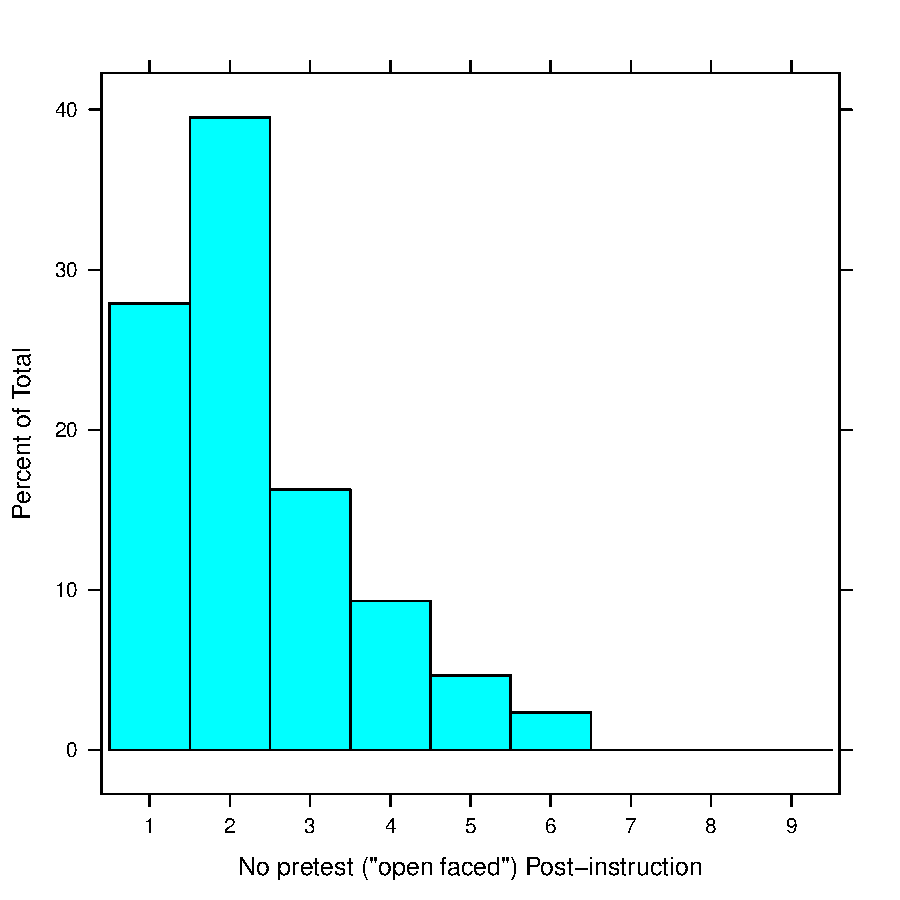
\includegraphics[width=0.5\textwidth]{hypotheses-surprisedistributions1.pdf}}
    \subfloat{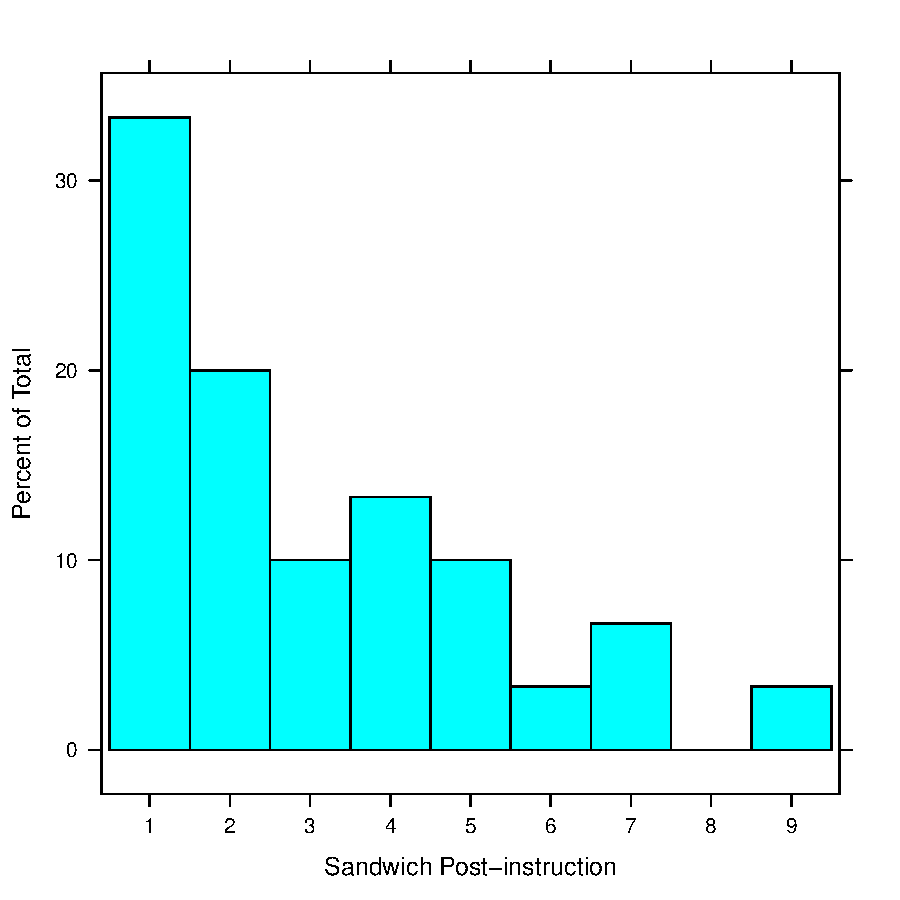
\includegraphics[width=0.5\textwidth]{hypotheses-surprisedistributions2.pdf}}
    \caption{Distributions of surprise ratings for the sandwich and open-faced
        groups, note the slight increase in ``1'' ratings (which may indicate resistance
        to the intervention) co-occurs with an increase (from none) in ratings 7-9 in
        the sandwich group.}
    % For final, re-do these graphs so they have the same y-scales
\end{figure}

Note, I suspect it is unlikely that individuals experienced the same kind of
``visceral'' surprise from the blurb that can be obtained by, for example,
statistics we've used regarding things like abortion and the death penalty. And,
while it may be due to a limitation of imagination, I have difficulty imagining
an evolution item that would elicit this kind of surprise.

In addition, we replicated the relationships predicted by the RTMD theory in
another population. Confirmatory factor analysis yielded quite similar results
to simple correlation tables between the means of attitude-relevant items. In
particular, all proximal relationships held in this population (those
represented by lines in Figure~\ref{fig:rtmd}) and in each survey, either 12 or
13 out of 15 total relationships were in the direction predicted by RTMD. Less
formally, it appears that the correlations between evolution and climate change
increased after our intervention---perhaps indicating a shift in which
participants viewed climate change as part of ``real science.'' Similar
increases in anti-correlation with nationalism were observed. However, we have
not yet established appropriate statistical machinery to test the significance
of these effects.

\subsection{Discussion}

In general, we have established quite clearly that individuals are largely
ignorant of the mechanism via which greenhouse gases cause global warming,
suggesting that this is a reasonable object of study! More specifically, even
this (relatively dry) 400-word blurb was able to effect shifts in attitudes and
elicit non-trivial surprise ratings from individuals. It remains to see how
attitude shifts and learning are related, but the results as they are seem
sufficient basis for proceeding on an educational research program including
mechanism!


% This should be placed in the correct location above

\begin{figure}
    \begin{center}
        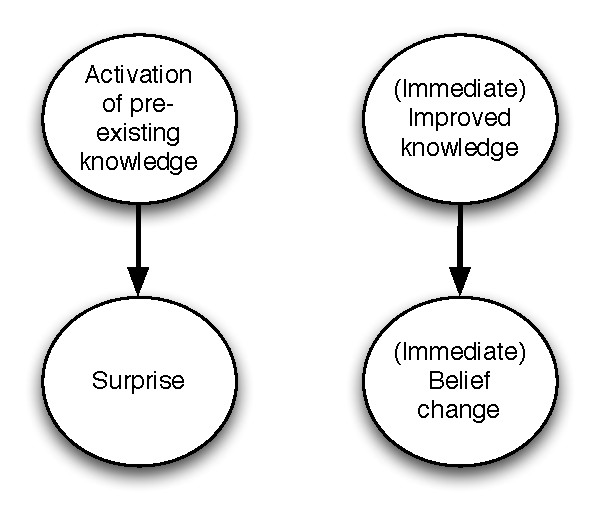
\includegraphics{causal2.pdf}
    \end{center}
    \caption{A graphical model representing the relationship between forms of
        psychological processing of factual information observed in
        chapter~\ref{chap:mechanism}. Here, the relationship between pre-existing
        information and surprise was the result of an experimental manipulation and
        is assumed to be causal.}
    \label{fig:causal-mechanism}
\end{figure}

\section{A web-based intervention with UC Undergrads}

Given the replicated demonstrations of significant attitude changes described
above, we proceeded to assess whether the mechanism-explanation effects we had
obtained were durable rather than transient. This study extended prior work by
delaying the post-test several days. We also wondered whether an ``experimental
demand'' from the classroom setting might have driven our prior results, so we
provided the intervention on-line; that is, we assessed whether our materials
would elicit significant attitude change even though students participated via
their own computers, without experimenter observation. Thus we concurrently
explored the longevity (via delay) and format (on-line) aspects of our
phenomenon. We also extended our prompts to incorporate more demographic and
introspection queries.

\subsection{Methods}

The survey and instructional materials were those reported in Ranney et
al. (2012a \& 2012b; the latter includes the full 400-word text of our
intervention). The primary difference was that administration was conducted
entirely online, via the Qualtrics Inc. (Provo, UT) system. Eight items were
added to pre- and post-test attitude surveys to add reliability to the related
RTMD metrics (specifically, national and religious affinities; these metrics
will be reported elsewhere). Five further questions were introduced immediately
following the instructional material to elicit introspection (about
embarrassment, disagreement, etc.).  Undergraduates (N=80) were recruited via
the Research Participation Program (RPP), administered by the University of
California, Berkeley (UCB) psychology department. Such recruitment allowed us to
administer a pre-test to about half of the students (38) between 8 and 26 days
($\mu=18.5$ days) before any of the 80 participated in the study, which may have
allayed test-retest effects (although Ranney et al., 2012a, found little
evidence for them). Thus, as with Ranney et al. (2012a), some participants
received the full survey testing ``sandwich'' while others had no pre-test. A
delayed post-test was given to all participants between 1 and 8 days later
($\mu=4$ days). This range was used to assess the timecourse of retention in
planning subsequent studies, We lack the power to test forgetting over time here
(though numerically, did not observe any!).

\subsection{Results and Discussion} 

Split this up! Note results have changed a bit for Knowledge (both kinds) using
regression and glht. Should also do something more definitive with the GW
attitude data (though this was unchanged for the CogSci paper).

In general and as anticipated, we replicated Ranney et
al.’s (2012a) results and extended them by finding that shifts were retained
over the mean (four-day) delay. 
% Include more verbiage here explaining lme4, Anova and glht
Scored knowledge was comparable to previously
tested UC students, rising from 3.8 on pre-test to 6.5 post-test and 6.3 on
followup (gains from pre-test were significant at $p<0.0001$ for both subsequent
scores). GW belief ratings (with higher ratings being
more in concert with science’s consensus) increased from a 6.20 pre-test mean to
a 6.54 post-test mean ($t(79)=2.5, p=0.006$; a healthy improvement on our 1-9
Likert scales!). Some of this improvement
diminished over the following days, but most was retained: the mean score on the
delayed post-test was 6.44 (t(79)=1.7, p=0.05). Self-rated knowledge means
increased markedly from pre- to post-test (4.5 to 5.6 on a 9-point scale,
t(79)=8.5, p<0.001). Retention of this increase, gratifyingly, was also noted on
the delayed post-test (5.2, t(79)=6.2, p<0.001). (The immediate increase in
self-rated knowledge, in fact, replicates results from the ``sandwich''
interventions in Ranney et al., 2012a, though those results were not reported.)

\subsubsection{Micro-analysis of GW ratings}

Table~\ref{table:uc-online-gw-means} reports the mean rating across participants
for agreement with individual items (For the full text of these items, see
Appendix~\ref{app:survey-items}). The largest gains were found in agreeing with
``Human activities are largely responsible for the climate changes\ldots'' (a
0.25 gain) and certainty that global warming is occurring (a 0.19 gain).  In
general, gains were fairly consistent across all GW measures, ranging only
down to 0.11 at the lowest (the über-greenie “humans are severely abusing the
environment”). Interestingly importance of lifestyle changed the most
(0.27, though this was not included in the tested average gw variable).
Expectation of engagement, dishearteningly, clocks in at a 0.05 \emph{drop}! 
% Enter motivational interventions like Oroeco?

% latex table generated in R 2.15.1 by xtable 1.7-1 package
% Thu May  9 12:43:59 2013
\begin{table}[h]
\caption{Mean GW ratings, online with UC undergrads} 
\label{table:uc-online-gw-means}
\centering
\begin{tabular}{>{\sffamily}rccc}
  \toprule
 & pre-test & post-test & followup \\ 
  \midrule
  gw1\_2 & 6.61 & 6.86 & 6.36 \\ 
  gw2\_1 & 5.19 & 5.31 & 5.25 \\ 
  gw2\_2 & 6.61 & 6.81 & 6.67 \\ 
  gw2\_3 & 5.81 & 5.97 & 5.97 \\ 
  gw2\_4 & 6.78 & 6.86 & 6.67 \\ 
  engage & 5.91 & 5.86 & 6.11 \\ 
  lifesty & 4.83 & 5.11 & 4.94 \\ 
  \bottomrule
\end{tabular}
\end{table}



\subsubsection{Correlations}

Scored knowledge and self-rated knowledge are significantly correlated pre-test,
so participants have decent meta-cognition here.
% TODO: insert statistics from Retention notebook in RPP_Su2012

\subsection{Interim conclusion}

In sum, this study extends the finding that well-considered information, even
received online, increases anthropogenic global warming acceptance and
behaviorally relevant attitudes; the conceptual changes that result from reading
even 400 words have notable longevity. These effects have been replicated with
members of the general public as well (unpublished data). Computer-based
interventions often scale well, enhance reliability, and prove cost-effective;
given our results, we recommend the online distribution of mechanistic
explanations, especially about climate change.  

% Currently, this is just significant results for the UC CogSci class (2010?)
% from “general improvements”
\extrarowsep 5pt
% copy pasted from mechanism/uc-classroom-summary.csv
% siunitx seems to be doing fine, but you can set it up like this if desired:
% \sisetup{round-precision=2,round-mode=figures,scientific-notation=true}
% I like table-parse-only. This doesn't work somehow: [table-number-alignment = center]
\begin{longtabu}{X[2.5]S[table-parse-only]X[l]}

% Final \\ necessary to compile!
\caption{Summary of results for college classroom interventions \label{table:summary-classroom}}\\
\toprule
Result & {$p$-value} & Statistic \\ \midrule
\endfirsthead

% The empty option prevents a TOC entry from being generated
\caption[]{College classroom interventions, continued}\\
\toprule
Result & {$p$-value} & Statistic \\ \midrule
\endhead

\bottomrule
\endfoot

People don't tend to mention the mechanism in pre-test (11/42), but they do in
post-test (S post is 26/30, N is 39/43 - stat computed for S group pre- vs.
post-, which has a lesser prevalence of mech than N) & 3.20E-07 &
Fisher's exact "two-sided" \\
Misconceptions are common in the pretest but not the post test, total 0.38 pre-
to 0.10/0.12 (S/N) post-test. Ozone .19 to .03/.02 (S/N),  wrong GHG  .24 to
0.07/0.09 (S/N). (test on total misconceptions, S pre- to post-test) & 0.01
& Fisher's exact "two-sided" \\
Participants don't mention energy leaving the earth until prompted.
Specifically, of the four codes that deal with this topic, only 6 mention
something about "trapped heat" in the pre-test on the first (i.e., the only
unscaffolded) question. & 0.0002 & Fisher's exact "two-sided" \\
Use of infrared is greater post-test than pre-test. Goes from 0 to 16 / 22 in S
/ N groups. & 3.50E-08 & Fisher's exact "two-sided" \\
S: GHG Objecive knowledge scores improve after the blurb & 5.08E-05 &
$t(29) = -4.75$ (paired) \\
N: GHG Objecive knowledge scores improve after the blurb & 2.00E-06 &
$t(78.2) = -5.14$ (Welch) \\
S: Light Objecive knowledge scores improve after the blurb & 3.94E-07 &
$t(29) = -6.51$ (paired) \\
N: Light Objecive knowledge scores improve after the blurb & 1.20E-04 &
$t(79.02) = -4.06$ (Welch) \\
S: Energy Objecive knowledge scores improve after the blurb & 0.04 &
$t(29) = -2.15$ (paired) \\
N: Energy Objecive knowledge scores improve after the blurb & 4.60E-04 &
$t(80.82) = -3.6547$ (Welch) \\
Differences in GW attitudes are significant & 0.013 & $t(72) = -2.28$
(paired / imputed) \\
S pre- to post-test: Increase in self rated knowledge is highly significant
(actually in hypotheses.pdf currently) & 1.40E-05 & $t(29) = 4.96$
(paired) \\
N post-test (compared to S pre-): Increase in self rated knowledge  is highly
significant (actually in hypotheses.pdf currently) & 0.014 & $t(78.7) = 2.23$ (Welch) \\
N post-test (compared to S pre-): Increase in self rated knowledge  is highly
significant (actually in hypotheses.pdf currently) & 0.014 & $t(78.7) = 2.23$ (Welch) \\
N post-test (compared to S pre-): Increase in self rated knowledge  is highly
significant (actually in hypotheses.pdf currently) & 0.014 & $t(78.7) = 2.23$ (Welch) \\
N post-test (compared to S pre-): Increase in self rated knowledge  is highly
significant (actually in hypotheses.pdf currently) & 0.014 & $t(78.7) = 2.23$ (Welch)
\end{longtabu}

% New results not in CogSci paper yet

\section{A web-based intervention on Amazon Mechanical Turk}

\subsection{Notes to integrate}

A number of additional concerns arise at this point. People may try to take the
survey again, they may lie about their demographics (i.e., claiming they are
U.S. residents so that they may gain the credit), and (bizarrely, as this does
not reduce time required, or increase payment) they may copy and paste from
online sources. Myles (so far) has identified line 14 on his sheet as a problem
in this regard.

\section{Summary and Conclusions}

We've shown across a number of populations that ignorance of the basic
physical/chemical mechanism of the greenhouse effect is rare. Across a variety
of intervention styles, we have shown that individuals are able to markedly
increase their abilty to describe the greenhouse effect, and that such an
intervention additionally shifts climate-related beliefs and attitudes.
400-word mechanism description

%TODO - things we can really address with the followup data:

Look at the relationship between folks saying they learned / were surprised /
stuff was knew on the basis of their scored knowledge. This is an argument
against the notion that folks knew things already, but didn’t think to mention
them given our prompts.

\section{Acknowledgements}

The work reported in this chapter has been previously published, in part, in
\textcite{ranney_why_inpress,and_others}. It is re-used here with their
permission, and the permission of the publishers.

% \graphicspath{{two-routes-estimation/}}

\chapter{Two Routes to Improved Numerical Estimates}
\label{chap:two}

As described in Section~\ref{sec:two}, cognition can occur in a relatively local
or special-purpose manner, or alternatively in an integrated fashion that (among
other things) affords volitional or conscious access. In
\cite{clark_known_2010}, we provide some preliminary evidence and argumentation
for separable learning processes which might be differentially involved when
learning numerical information. Below, I present an overview of two experiments
in abbreviated form, noting those details that are relevant to the questions
posed above. Specifically, these results demonstrate our ability to observe, and
potentially guide cognition between heavily conceptual \emph{episodic} or
\emph{semantic} modes of operation on one hand, and less conceptual emotional
processing on the other.

\section{Overview}

In short, participants saw textual descriptions of numeric items and provided
their best estimate. After this, they received the true value, and indicated the
degree to which they found the true value \emph{surprising}. After a period
including at least one night's sleep, participants were presented with the
previously shown textual descriptions.  Here, participants indicated their
\emph{metacognitive assessment of their memory} from the item from the day
before, in addition to re-estimating (or potentially recalling) the value.

\section{Experimental Methods}

The following experiment was designed to assess whether estimative improvement
occurs even with respect to items for which no feedback was received---as was
found in curricular NDI studies
\cite[e.g.,][]{munnich_numerically-driven_2004,ranney_designing_2008}. The
experiment (1) addresses the effects of surprise and the timing of feedback on
subsequent improvements in numerical estimation---as well as (2) probes whether
these improvements are necessarily mediated by explicit recollection. A subset
of the EPIC procedure was used to explore these issues; participants engaged
only in estimation (``E'') and feedback (``I''), leaving aside personal
preference (``P'' and ``C''). 

\subsection{Participants}

Twelve people (seven female) participated, including UC Berkeley undergraduates
and members of the general public recruited via online recruitment systems (RPP
and RSVP). They received either course credit or \$20 for their participation in
two one-hour sessions over two consecutive days. Ages ranged from 18-56 years. 

\subsection{Materials}

Numerical facts (106 of them) were selected from \citeauthor{ranney_designing_2008}
. An example is ``The current percentage of deaths in the U.S. that are
caused by lung cancer.'' Three statistical facts were set aside for the basis of
example items (namely US population, world population, and US Gross National
Income). Items ranged over a number of topics, and included politics, population
dynamics, economics, the environment, education, crime etc. Most items were
expressed in percentage form, with the rest being counts of dollars, people,
events or things. For numbers above 999, a comma was used, as in ``13,600.''  For
numbers in the millions, billions, or trillions, the appropriate word was used
to indicate the order of magnitude (e.g., ``300 million'').  This was intended to
minimize possible confusions about the exact value of the number.

\subsection{Procedure}

Custom software utilizing Vision Egg \cite{straw_vision_2008} presented all materials and
collected responses. (Source code available upon request,)  Descriptions of
numerical facts were presented in 1-4 lines of text (with less than 55
characters per line). A prompt for numeric entry was located below the
description. Feedback concerning the veridical value was provided in a third
location, between the description and the text-entry area.

\subsubsection{Blocks of Items}

Items were randomly distributed into the following four kinds of blocks. Each of
these blocks was involved in two or more runs over the course of the experiment.
E: Participants only provided Estimates in a single run. EI: Participants
provided Estimates followed immediately by correct numerical Information as
feedback (i.e., feedback was provided in the same run as the initial
estimation). E\_I: Participants provided Estimates, then received correct
numerical Information in a run that was well-separated from the run in which
they provided their Estimate (i.e., ``\_'' signifies a temporal delay). New: A
block of items was reserved in both experiments to provide a gauge of false
recognition or false recollection.

\subsubsection{Experimental Runs}

Participants engaged in a number of self-paced runs on each of the two
consecutive days, as figure~\ref{ei-procedure} depicts. The presentation of
stimuli and responses made were uniform across a given run. During the first
day, analogous to a ``study'' phase, participants completed three partially
similar runs of numerical estimation and/or informative feedback. The second day
was analogous to a ``test'' phase, in which participants’ learning was assessed.

 
%% This probably doesn't go here
\begin{figure}[h]
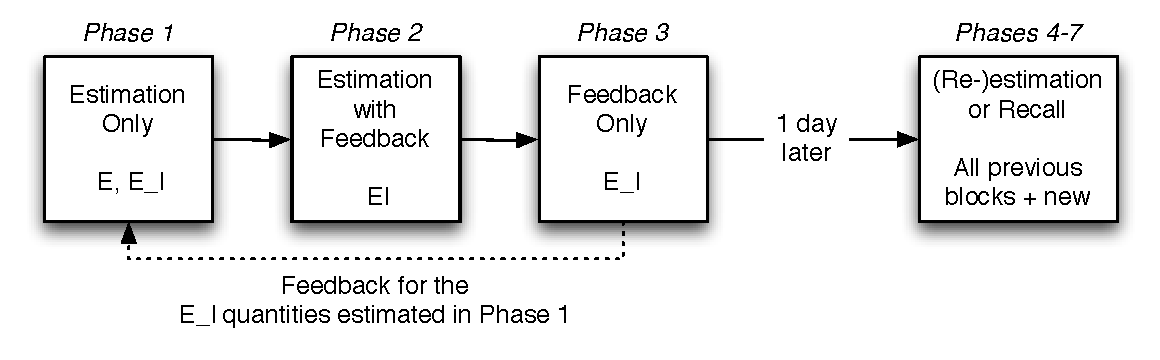
\includegraphics[width=\textwidth]{Experiment1-procedure.pdf}
\caption{A schematic of the experiment's seven runs. Run 1:
Estimates were obtained for the E and E\_I blocks of items (23 each), randomly
intermixed in one run. Run 2: Participants provided 23 Estimates that were
immediately followed by Informing the participant of the correct value. Run 3:
Feedback (I) was provided for the 23 items from the E\_I block that had been
Estimated in Run 1. Runs 4-7: Subjects estimated (or recalled) quantities and
provided explicit memory ratings for all previous items as well as 34 new
items.}
\label{ei-procedure} 
\end{figure}

During estimation (Runs 1 and 2, with 23 items each), subjects were given a
textual description of an item's quantity, followed by a prompt to provide an
estimate. For Run 2, feedback was provided 500 milliseconds after each estimate
was entered. For Run 3 (with 23 items), the correct numerical value was provided
prior to the textual description in order to minimize covert estimation.

In Runs 2 and 3 (thus, for blocks including ``I''), surprise ratings were elicited
regarding the values given as feedback. Three possible levels of surprise were
collected: 

\begin{enumerate}
\item Little or no surprise
\item Genuine surprise
\item ``Visceral'' or intense surprise
\end{enumerate}

On day 2, trials were similar to the estimation-only trials in Run 1 described
above---no additional feedback was provided. An additional 34 items from the
``new'' block were randomly intermixed with the items presented during study.
Additionally, participants rated their memory for the item according to the
following 4 levels: 

\begin{enumerate}
\item ``The item is new to me'' 
\item ``The item was presented yesterday, but I have no sense of the value 
provided as feedback'' 
\item ``The item was presented yesterday, and I have some sense of the correct value''
\item ``The item was presented yesterday, and I have a fairly accurate recollection of
the value.'' 
\end{enumerate}

Choice 1 indicates no recognition or recollection.  This is equivalent to
labeling the item as ``new,'' and it is the correct response for items from the
new block.  Choices 2-4 as a group indicate that the item is ``old,'' but with
varying levels of familiarity and/or recall.  These are correct responses for
the E, EI and E\_I blocks (although choices 3 and 4 entail a belief that the
participant actually received feedback at study, and so might also be considered
incorrect for the E block). Choices 2 and 3 indicate perceived recognition, but
at least a partial failure in recall.  Choice 4 indicates a subjective sense of
fairly complete recall.

Note that the estimation task used here is somewhat different than item
recognition or cued recall tasks used in many learning and memory studies. The
closest point of comparison is likely the notion of \emph{source} memory, in
which details surrounding the initial experience of the experimental item are
well correlated with hippocampal activity at encoding
\cite{davachi_multiple_2003}. In particular, we are \emph{not} asking
participants to attempt to recall a particular item from memory, Indeed, these
memory ratings can be viewed as a form of metacognition regarding the estimation
process and it's relationship to the participants previous experience with the
item (i.e., source memory for the item).

\subsection{Analysis}

We modeled improvement as a binomial outcome \cite[as
did]{munnich_longevities_2005}. This allows for the treatment of items that have
differing distributions within a unified framework (e.g., a linear model would
have difficulty modeling both percentages and values in the billions,
particularly given our sample size).  Items were labeled as to whether estimates
improved or not. These labels were fit with a binomial generalized linear model,
using the lme4 package in the R statistical environment
\cite{r_development_core_team_r:_2009_fixed}. This treatment allows for a full
multi-factorial mixed-effects analysis. Below, participants are always included
as a random effect, and other factors are treated as fixed effects. Linear
contrasts were evaluated using the multcomp package, which controls for
family-wise error rate \cite{hothorn_simultaneous_2008}.

Unless otherwise noted, data were pre-processed to remove ties. This was done to
allow for a null hypothesis that 50\% of the remaining items randomly improved
and 50\% randomly worsened. If we counted ties as failures to improve, then
random drift would end up spuriously suggesting the lack of an effect. Removing
ties allowed for tests of whether estimates improved, on average, more than they
worsened––both formally and when examining graphs. Otherwise, the removal had
little effect on the results, except where explicitly noted below.

%% Include a simplified figure for experimental design
% I need to redo these results (using Sweave) and carefully explain which items
% were excluded

\section{Results}

\subsection{Improvements in Accuracy of Estimation}

We can easily reject a null model in favor of a model predicting different
improvements across ``I,'' ``EI,'' and ``E\_I'' feedback conditions ($\chi^2(2)
= 25.9, p < 10^{-6}$). Post-hoc comparisons between each condition and chance
levels, as well as between condition comparisons (as in a Tukey HSD test) were
performed simultaneously. 
% For this document, it would be good to give the full explanation including
% lme4, glht, etc.
In the no-feedback case (E), estimation improvement
did not differ significantly from chance ($p = 0.39$), although improvement with
Immediate (EI) and Delayed (E\_I) feedback were clearly above chance ($p <
10^{-4}$). This may seem unsurprising, but it might have been the case that
improvements were at least partially driven by general improvements in
estimation skill, and this would have led to at least some modest improvements
even without feedback on test items. Indeed, this kind of skill development was
the successfully accomplished goal of various EPIC-based curricula
\cite[e.g.,][]{munnich_numerically-driven_2004,ranney_designing_2008}. In this
less extensive experimental manipulation, though, we understandably elicit no
such skill improvements. Thus, we assume that these improvements are driven
almost entirely by item-specific learning.

\subsection{Predicting learning from surprise and meta-cognitive memory
assessment}

As is often the case, the participants' forced familiarity judgments appeared to
be superior to their own assessment of their memory.  In participant
debriefings, several individuals claimed to be uncertain whether items were old
even from Run 1 to Run 3 for items in the E\_I block––that is, over an interval
of less than 30 minutes!  However, participants were excellent at discriminating
between old and new items a day later when given a forced choice; 76\% of new
items were identified as new on Day 2, compared to an average of less than 9\%
regarding previously seen items. This level of recognition accuracy is not
surprising given the considerable depth of processing involved, and the rich
pre-existing memory structures available for scaffolding these episodes.

\begin{figure}[h]
\centering
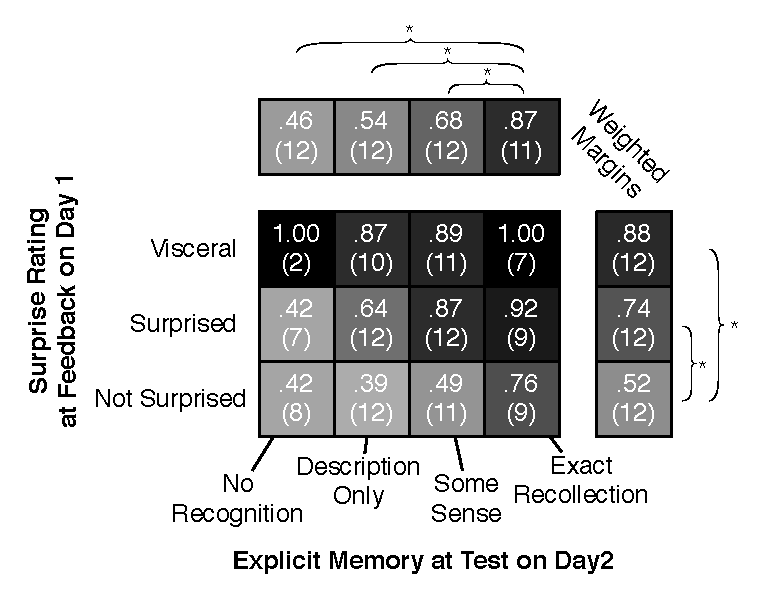
\includegraphics{shaded-table-reversals.pdf}
\caption{Fraction of items improving across different levels of surprise rating
and metacognitive memory assessment. The number is parentheses represents the
number of subjects (out of 12) contributing to that cell. Margins are
appropriately weighted according to the number of items in each bin, and as such
are not the simple mean of the row or column in the central table. Significant
differences between levels of individual factors are marked with an asterisk.}
\label{ei-table} 
\end{figure}

As the lack of feedback yielded non-significant changes in estimation accuracy,
here, we consider only items from conditions including feedback (``I''). These
effects are depicted in Figure 3.  A model that predicts estimation improvements
on the basis of both surprise and declarative memory responses is well-supported
by the data. We readily reject a reduced model excluding memory ($\chi^2(3) =
34.8, p < 10^{-7}$), as well as one excluding surprise ($\chi^2(2) = 295.22, p <
10^{-16}$). An inclusion of an interaction term does not yield a significantly
better model ($\chi^2(6) = 2.85, p = 0.8$). 

% Test for this is in surprise.diff.by.condition function in pilot2 dir
It should be noted, that there is a small (but non-significant)
difference in surprise ratings between EI and E\_I blocks: subjects rated 64\%
of EI block items as surprising (``2'' or ``3'') vs. 59\% for E\_I (although no
straightforward effect was observed with metacognition on memory).  This result
mirrors the result obtained in the above study on climate change cognition, in
which prior estimation increased participant reports of surprise
\cite[cf.][]{rinne_estimation_2006}.  Thus, the
timing of feedback may have an effect on estimation improvement that is mediated
by surprise; these issues seem best addressed in a subsequent study, though.
Below, we only consider comparisons within surprise level and memory ratings
independent from one another.

Recall of the exact value (memory response ``4'') as compared to other memory was
a highly significant predictor of improved estimation (all $p$'s $< 0.001$ for the
lower two ratings, $p = 0.01$ when compared with response ``3''). No other
comparisons between memory levels are significant. For surprise, both moderate
and visceral ratings yielded significantly greater improvement than for
no-surprise rated items ($p < 0.002$ in both cases), but did not differ
significantly from one another. Note that participants provided the exact
numerical figure given as feedback only 35\% of the time when selecting choice
4. Even if we broaden this liberally to items where participants are within 15\%
of the true value, they were only correct about 74\% of the time.

Finally, if we consider the relation between surprise and metacognition on
memory, there
appears to be very little correlation. The correlation of fixed effects between
memory and surprise terms in our model was consistently smaller in magnitude
than 0.1. This, combined with the lack of significance of an interaction term,
provides some evidence for independent learning processes.

While both \emph{surprise} and \emph{metacognitive memory assessment} were
predictive of improved estimation from the first to the second session, these
measures did not interact significantly, and moreover were uncorrelated with one
another (i.e., progressive darkening from the lower-left to upper-right corner
in Fig.~\ref{ei-table}).

%% I have re-run correlations between surprise and metacognition using
%% tetrachoric methods. Looking at the data though, it seems that I should
%% probably employ something like a chi-squared model. I suspect the rows do NOT
%% have identical frequencies, and that visceral surprise does reduce the
%% likelihood of a "new" response

On it's own, this result would be insufficient to make strong claims about
multiple cognitive routes for learning. But, this result fits well with an ever
increasing literature (an overview of which was provided in
section~\ref{sec:two}). 

\subsection{Exclusions}

As many as three items lacked estimates from some subjects or exhibited a clear
lack of understanding (e.g., a number such as 10 million for a question asking
for percentage) and these items were excluded from the analyses above. Due to a
technical issue, participant 01 was not run on the standard E manipulation, but
was included in memory and surprise-related analyses, as these analyses did not
include E trials.

\section{Discussion}

Given the overall improvements in estimation ability evidenced in curricular
studies by \citeauthor{munnich_numerically-driven_2004} and
\citeauthor{ranney_designing_2008}, it is of interest that we see no statistically
significant improvement in items that didn't receive feedback (the ``E'' block).
In other words, it appears that participants did not improve their estimation
skills in the absence of feedback particular to a given item.
Nonetheless, it seems that learning in this considerably shorter experiment was
largely item-specific and related to the integration of feedback. This lack of
improvement in the present experiment may be due to a lack of time for
reflection or development of strategies––which were highlighted, taught, and
fostered in the curricular studies.
(\nptextcite{munnich_numerically-driven_2004,ranney_designing_2008} also focused, to
a fair degree, on preferences and personalized policies which may engage a web
of related concepts.)

\subsection{Learning Without Metacognitive Report of Recall}

From the point of view of a memory theory, the most interesting result is
perhaps the existence of learning even when participants claimed “no sense” of
the numerical value provided at feedback---rather like a memorial analog to
blindsight. This argues against the notion that improvements in estimation are
simply the result of explicit episodic memory. The result is reminiscent of
extant dual-process memory models.  For example, \citeauthor{davachi_multiple_2003}
suggest that successful recognition could occur through a process of
recollection and/or a sense of familiarity.  These processes moreover appear to
be subserved by distinct sub-regions in the medial temporal lobe.  In the
present study, though, we see improvement in numerical estimation---which is
perhaps most akin to a cued recall task for EI and E\_I items---without full
recall of the number presented on the previous day.  Thus, the task here is
perhaps more naturally expressed in the language of the remember/know
distinction \citeauthor{knowlton_relationship_1998}.  That is, while participants
appear not to remember a specific (usually multi-digit) number from the previous
day, there is still a sense in which they know the number better than they knew
it the day before.

Based on the significance of the existing results, however, it seems reasonable
to posit that a non-episodic form of learning undergirds some of the improvement
in participants’ abilities to estimate accurately.  Further, the learning for
improved estimation (or memory) seems to occur often without an explicit, precise
recollection of the feedback from the prior day.  This argues for some implicit
and/or rapidly semanticized learning in support of these improvements. In
particular, this appears to have something of a ``less conceptual'' flavor.
This line of reasoning is reminiscent of studies of children applying abstract
mathematical rules before they are aware of doing so
\cite{siegler_unconscious_2000}.

Of course there is also a clear role for explicit episodic recall in learning
numerical information. In particular, how well participants believed they could
recall the number was indeed predictive of improved estimation. But
instructional materials that elicit surprise in students may allow students to
learn without conscious awareness that they have learned anything---at least in
domains that are scaffolded by nontrivial preexisting knowledge. If the material
is unsurprising, it appears that episodic encoding may be a critical step in
successful improvement. It should be noted that surprise might be too specific a
notion. It may be that the relevant feature has more to do with general
emotional salience, or how interesting the material is to students. Certainly,
however, it seems that there are multiple routes to learning even relatively
concise facts. Thus, our development of climate change interventions might
usefully engage factors such as surprise and engagement with pre-existing
knowledge to bolster more rote forms of learning.

% This should be put in the appropriate place above

\begin{figure}
\begin{center}
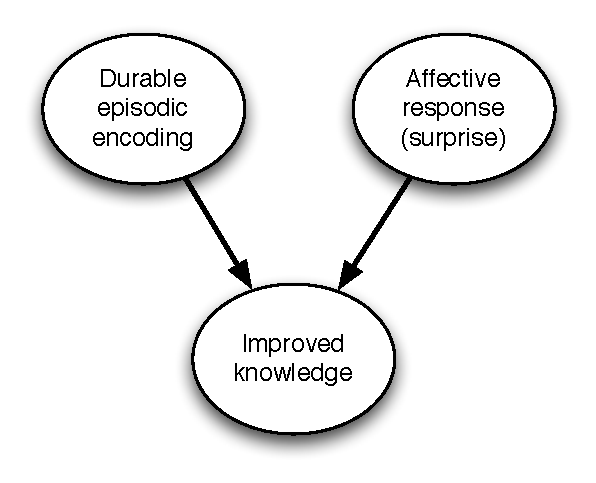
\includegraphics{causal1.pdf}
\end{center}
\caption{A graphical model representing the relationship between forms of
    psychological processing of factual information observed in
    chapter~\ref{chap:two}. Arrows represent conditional probability
    relationships and \emph{not necessarily causation}.}
\label{fig:causal-two}
\end{figure}

% \graphicspath{{pro-ndi/}}

\chapter{Learning Representative Climate-Relevant Numbers}
\label{chap:prondi}

Notes - contrast with mechanism study. Much less scaffolding, more burden on the
student to make sense, more burden on instructional design to make things clear.

\section{Actual Abstract (delete heading before submission)}

\section{Altering Beliefs with Factual Numbers}

This came from the CogSci 2013 paper - edit or cut

The Numerically-Driven Inferencing (NDI) paradigm has yielded marked
attitudinal and conceptual shifts with quite minimalist interventions. NDI and
one of its procedures, EPIC (both introduced by Ranney and colleagues in 2001),
represent a particularly compact, well-specified intervention. In EPIC,
participants (1) provide an Estimate for each policy-relevant item’s quantity;
(2) state a preferred target (or monetary allocation) Policy (or Preference) for
each quantity; (3) receive actual quantities as feedback to Incorporate (as new
``Information''); and (4) indicate whether one’s policy has Changed upon receiving
feedback. With even a single well-selected quantity, the EPIC procedure’s
feedback often shifts participants’ attitudes. Conceptual changes resulting from
EPIC are often remarkably durable for such a minimal intervention (e.g., Ranney
et al., 2008), as evidenced by increased estimation accuracy up to 12 weeks
after the procedure (Munnich, Ranney, \& Bachman, 2005). Therefore, we sought to
employ NDI interventions in addition to the mechanism intervention from Study 1
and before. Specifically, we presented different participant groups with
numerical information that is relevant to global climate change acceptance. We
used numbers that were likely to boost acceptance (Study 3), as well as numbers
that we thought might erode individual's belief in climate change (Study 2).

As before, survey methods employed in the following studies are described in
detail in Section~\ref{sec:survey}.

\section{Study 1: Online experiment with UC Undergrads}

Given the efficacy of “evil” numbers and previous successes of the NDI paradigm,
this study assessed the efficacy of numbers that support the claim of global
climate change. Again partly tongue-in-cheek, we call these “saintly” numbers.
Given prior NDI studies of similarly “shocking” magnitudes (e.g., Garcia de
Osuna, et al., 2004), our hypothesis was that the accurate feedback would
increase participants’ climate change acceptance, but diminish self-confidence
in their knowledge of the issue.


\subsection{Methods}

This study used an on-line version of materials, as did Study 1, and used a
UCB-RPP pre-test survey (completed by 30 participants) that yielded, on average,
an 18-day delay between pre-test and intervention. We queried individuals (N=60)
about eight quantities. The eight items included questions directed at
participants’ surprise and their reactions to each number (fictitious monetary
policies were left out of this version due to attitude shifts observed in the
simplified 8-item “evil” intervention). An added feature of the online
intervention is that we could remind individuals of the estimates they gave on
the same page on which they incorporated numerical feedback, ensuring that they
contrasted the two. As with Study 1’s online survey, an attitude and belief
post-test was administered immediately after our intervention and also after a
retention interval.


\subsection{Results and Discussion}

Attitudes, acceptance, and beliefs regarding climate change remained stable
after this intervention with “saintly” numbers (6.71 pre and 6.67 post). This
stability was unexpected (but see below for explanations), especially because
these items (as with the “evil items) were, as anticipated, able to
significantly erode self-rated knowledge (5.3 to 4.0, t(29)=-3.6, p<0.01). This
erosion was comparable to that found with the “evil” numbers. These items also
ranked relatively high on participant surprise compared to the 400-words from
Study 1. Mean surprise ratings across items was 4.8, while surprise ratings for
the 400 words was 2.9 (all ratings above “1” indicate some level of surprise).
% TODO: also include surprise for evil numbers here?

One of the most surprising numbers (at 5.2) was the percentage of active
researchers who support the tenets of anthropogenic climate change, reflective
of the strong relationship between perceived scientific consensus and acceptance
of climate change reported in Lewandowsky, Gignac, and Vaughan (2013). The two
numbers most comparable to the statistics in the 400 words were similarly
surprising, with the rises in atmospheric methane and atmospheric CO2 ranking at
5.9 and 5.1, respectively.

\emph{We can make a parallel here to Kahneman's pain studies / retrospective vs
experiencing.}

\subsubsection{Results on attitutudes}

In spite of these powerful impacts, in this study we observed no effect on
beliefs and attitudes. This lack of effect is counter to prior NDI studies, in
which individuals’ preferences and beliefs were often markedly shifted by even a
single number. An experimental silver lining here is the demonstration that
participants will not report greater climate change acceptance merely by dint of
experimenter demand! One possible explanation is due to a methodological change:
In prior NDI and RTMD studies, participants were explicitly told (a) that all
feedback statistics and other information were fully accurate (and that the
study involved no deceptions), and (b) the particular scientific/literature
source both for each statistic that was sought and each provided as feedback.
It is thus possible that participants were less compelled by the authority of
this study’s statistics, compared to those in Study 2.  Another possibility is
that, as in Study 2, participants were left feeling less knowledgeable—weakening
any boost these surprising numbers could have on climate change acceptance.
Individuals perhaps lacked an appropriate context for integrating this
information. The next study illustrates one way to contextualize such numbers.

\section{Study 2: Online intervention on Mechanical Turk}

Note that we did not include instructions to the effect that NO deceptions were
used.

Also - in both of the above studies, the inclusion of information about
authority was scant (e.g., “journal article” instead of PNAS).

% \graphicspath{{evil-ndi/}}

\chapter{Learning \texorpdfstring{``Evil''}{"Evil"} Non-Representative Climate Numbers}
\label{chap:evilndi}

The Numerically Driven Inferencing (NDI) is introduced in
Section~\ref{sec:ndi}. In Chapter~\ref{chap:two}, we
see that surprising numerical information can have a lasting impact on an
individual's conception of a politically relevant number--sometimes even without
conscious recollection of the experience that catalyzed this change.  Below, we
will see that misleading, cherry-picked numerical facts can have a marked shift
on individuals' beliefs and policy preferences. This result serves as a
call-to-arms for climate educators, as even relatively well-educated, liberal,
GW-accepting students are highly susceptible to the kinds of information
currently being used to undermine belief in climate change.

\section{Overview}

As described in Section~\ref{sec:comm-strategies},
there is some debate surrounding the value of scientific or numeric information
regarding climate change. Indeed, some have claimed that such interventions will
only serve to polarize individuals, thus making the situation worse than it
already is. However, some organizations publish out-of-context facts to try to
undercut the reality or gravity of human-caused climate change. Such numbers are
often blatantly cherry picked. For example, one con locate GW deniers who note
that the Earth’s temperature decreased (by 0.2°F) from 1940 to 1975
\parencite{jastrow_global_1991}. This surprising fact, though, hardly
contradicts the ever more obvious warming trend over the last 125+ years---one
can pluck many ``trends'' in noisy time series by picking endpoints that are
oddly high or low. Given this rather clear intent to mislead
\parencite[corroborated by][]{oreskes_merchants_2010}, we (partly
tongue-in-cheek) label these numbers ``evil.'' 

Our three hypotheses were that misleading facts would reduce:
\begin{enumerate}
    \item participants’ climate change acceptance, 
    \item ratings of their knowledge of the issue, and 
    \item their climate-change funding preferences.
\end{enumerate}
Of course, lest we would have eroded participants’ acceptance of anthropogenic
climate change more than fleetingly, we debriefed them right afterward with more
complete information---including a large dose of representative numerical facts
as well as the basic physical mechanism of GW (the mechanism is detailed in full
in Chapter~\ref{chap:mechanism}). It should be clear that we're not interested
in perfecting an approach to eroding acceptance of the overwhelming scientific
consensus on climate change! 

In this Chapter, we'll see easily obtained and dramatic effects with an
anti-climate NDI intervention. There is only one experiment reported, with the
intent of determining whether these materials would drive meaningful
changes. In particular, we administered this experiment only to undergraduate
seminar courses where we could be sure to administer a proper debriefing.

\section{Study: UC Classroom Intervention with \texorpdfstring{“Evil”}{"Evil"}
    Numbers}

\subsection{Methods} 
\label{sec:evilndi-methods}

\subsubsection{Participants}
\label{sec:evil-participants}

Two classes of UC Berkeley undergraduates (spanning cognitive science and
“Behavioral Change”) were engaged in this intervention ($N=104$). 59 students
completed the 8-item “no pre-test” version of the experiment and 45 completed
the 2-item full EPIC intervention. All participants were retained after
examining the coherence of survey responses.

In the 8-item intervention, 34 participants were female and mean conservativism
of 3.64 ($sd=1.59$). In the 2-item intervention, 31 participants were female and
mean conservativism was 3.68 ($sd=1.43$). Breakdown of political party is given
in Table~\ref{table:evil-party}.

% TODO: party table 
% latex table generated in R 2.15.1 by xtable 1.7-1 package
% Tue Jun 18 14:46:50 2013
\begin{table}[ht]
\caption{Stated party affiliations for participants in “evil” NDI study (UC
    Berkeley undergraduates).}
\label{table:evil-party}
\centering
\begin{tabular}{rrr}
  \toprule
     & 8-item & 2-item \\ 
  \midrule
  democrat &  20 &  21 \\ 
  republican &   4 &   2 \\ 
  green &   1 &   0 \\ 
  libertarian &   1 &   3 \\ 
  independent &   6 &   2 \\ 
  none &  21 &  13 \\ 
  other &   1 &   1 \\ 
  decline to state &   5 &   3 \\ 
   \bottomrule
\end{tabular}
\end{table}

\subsubsection{Materials and Procedure}

Participants were engaged in one of two similar misleading numeracy
interventions (depicted in Figure~\ref{fig:evil-flow}). In both versions, survey methods were as described in
Chapter~\ref{chap:survey}. This study utilized a somewhat compact version of a
pre- and post-intervention test using only the 14 items in
Table~\ref{table:rtmd-questions} (up through \textsf{engage}), plus a
self-rating of climate-change knowledge (for a total of 15).  
After the intervention, all participants also completed a brief demographic
survey. Notable results of this survey were reported above in
Section~\ref{sec:evil-participants}.

\begin{figure}[h]
    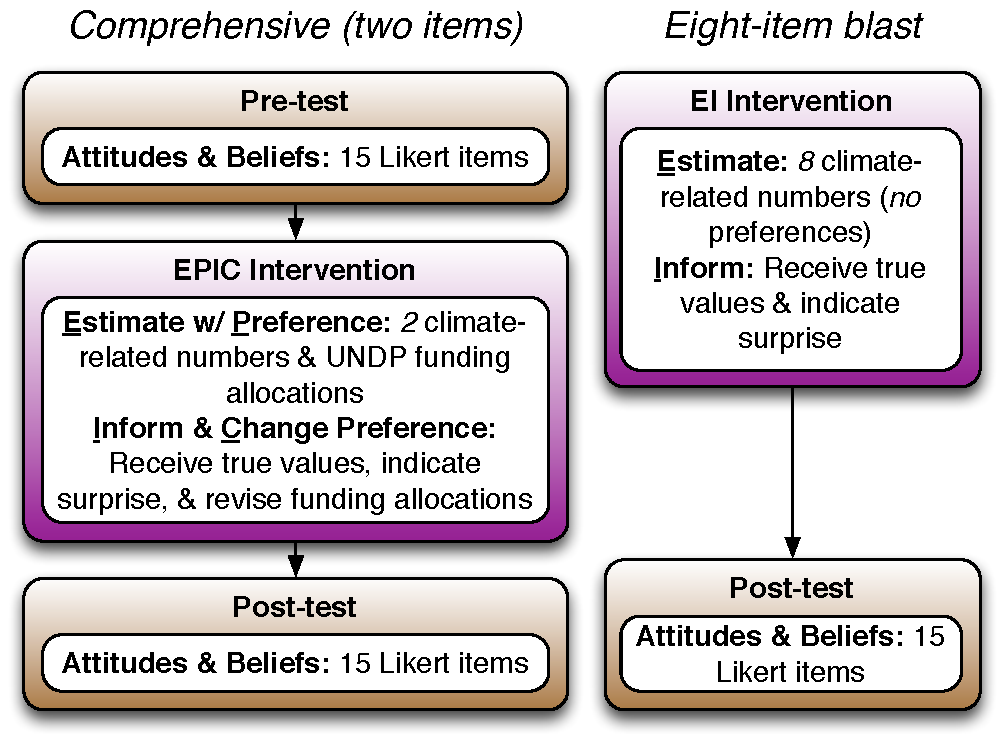
\includegraphics[width=6.5in]{evil-ndi-survey-flow.pdf}
    \caption{An overview of experimental flows for our “evil” NDI experiment. If
        we consider our EPIC or EI interventions to be “jam,” and our surveys to
        be slices of bread, we see that the participants in the 2-item condition
        recieved a full “sandwich.” (Participants in the 8-item condition
        recieved no pre-test).  Flow for NDI experiments in
        Chapter~\ref{chap:prondi} had a full “sandwich” structure, but used the
        greater bang-per-minute EI intervention style from the 8-item
        intervention.}
    \label{fig:evil-flow}
\end{figure}

In the “no pre-test blast” version of the intervention, participants estimated
each of eight items prior to receiving the feedback values, with an emphasis on
maximizing the quantity of feedback numbers presented to the participant. To
this end, this eight-item survey included only a post-test (i.e., no pre-test),
and lacked a policy component (thus, it was an EI intervention, lacking ``P'' or
``C'', simlar to the approach used in Chapter~\ref{chap:two}). 

A more comprehensive engagement containing only two items was administered to
the rest of the class. This version included a pre-test and additional questions
about each item. In addition, we asked students about their surprise level after
each feedback value and requested both their climate-change funding Policies and
post-feedback policy Changes versus various UNDP millennium goals.  Thus, this
latter variant was a full EPIC intervention. The same set of alternatives was
used across the 4 variants of the 2-item intervention, and these are listed
along with policy-relevant instructions in Appendix~\ref{app:undp}.

Note that while this experiment is presented first as a motivation for the
following chapters, it was actually carried out \emph{after} a number of
experiments in Chapters~\ref{chap:prondi} and \ref{chap:mechanism}. Thus, a
number of experimental design choices made here are motivated by findings from
experiments in those chapters.

\subsection{Results}

% TODO: Also note changes for each item / individual comparisons here (if you
% have time / people want)
Overall, these numbers had a profound impact, the details of which are described
below. As with other NDI interventions, and consistent with our pilot testing,
individuals generally found each of these items surprising, ranging from
surprise ratings of 5.83 to 8.53 across both interventions. Mean surprise
ratings were 6.03 for the 2-item intervention and 6.62 for the 8-item
intervention. Ratings were on a 1--9 scale, with all ratings above “1”
indicating some level of surprise.

\subsubsection{Shifts away from GW policy preferences}

As hypothesized, policy preferences for funding UN goals related to climate
change dropped ($\chi^2(1)=22$, $p<0.01$) for all eight funding priorities.
(Unfortunately for global warming as a social priority, the highest mean
pre-test preference for funding climate change initiatives reached only a 50-50
split of available funds.) These results are depicted in
Figure~\ref{fig:evil-alloc}. While, due to time constraints, we did not check
for a similar result in our 8-item intervention, it seems likely that similar
(or greater) shifts would occur along with the much more drastic GW attitude
shifts we'll see below.

\begin{figure}
    \centering
    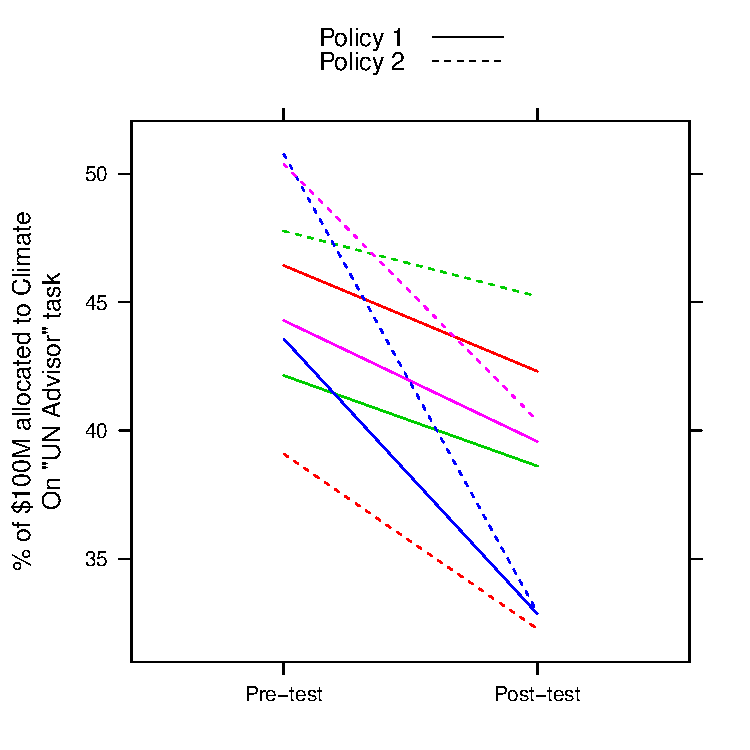
\includegraphics{evil-alloc.pdf}
    \caption{Significant drops in preference for allocation of \$100M towards
        climate-related projects on “UN Advisor” task ($p<5\times10^{-6}$). Each
        of the 4 survey variants is represented by a different color. The two
        policy choices remained the same (indicated by solid vs. dashed lines),
        while numerical information was varied across surveys. Values are
        expressed as a percentage of funds that were allocated to
        climate-relevant projects vs. projects supporting an alternative UNDP
        millenium goal.}
    \label{fig:evil-alloc}
\end{figure}

\subsubsection{GW acceptance eroded by misleading numbers}

Also, as hypothesized, mean climate change acceptance dropped significantly,
from 6.5 on the pre-test to 6.2 on the post-test for the two-item group (6\% of
available room, for a 9-point scale, $t(42)=-4.3$, $p<0.001$), and significantly to
5.9 for the eight-item group (12\% of available room, $t(88.6)=‑2.61$, $p<0.005$).
Note that these shifts were also in the direction of ambivalence (a ``5''
rating), and may reflect confusion rather than disagreement. Mean ratings are
depicted in Figure~\ref{fig:evil-GW}.

\begin{figure}
    \centering
    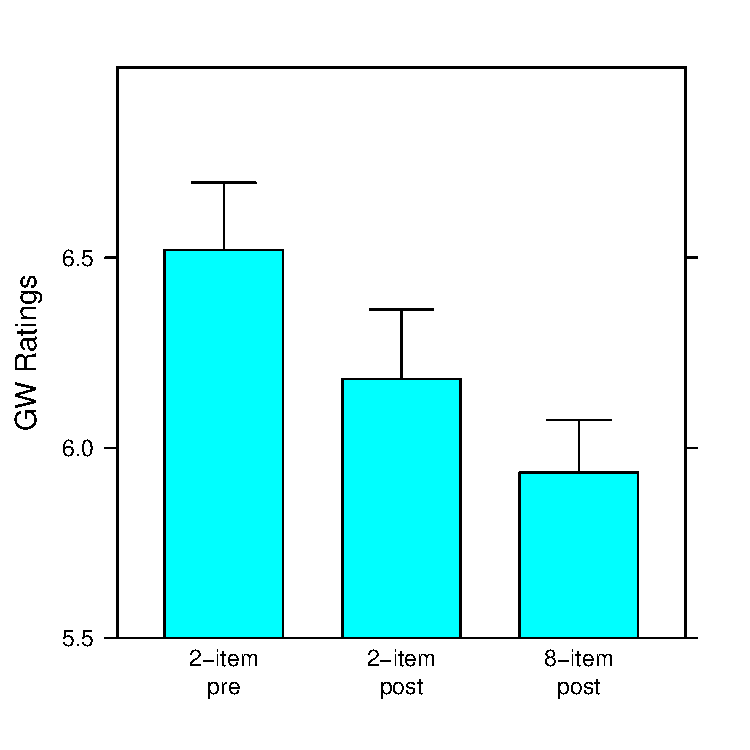
\includegraphics{evil-GW.pdf}
    \caption{Mean ratings for GW survey items on pre and posttest. Pretest
        surveys were only administered for the 2-item group, but should be
        indicative of population responses. Error bars represent standard errors
        for each measure.}
    \label{fig:evil-GW}
\end{figure}

\subsubsection{Self-confidence in GW knowledge eroded by misleading numbers}

Our third hypothesis was also supported, as self-rated knowledge dropped from a
mean of 5.0 on the pre-test to 4.5 for the two-item group (12\% of available
room, $t(44)=-2.5$, $p<0.01$), and plummeted to 2.9 on eight-item survey
($t(87.2)=-5.3$, $p<0.001$). This latter decrease, 2.1, represents 53\% of the
available room to drop on a 9-point scale, which is exceptionally large. These
ratings are depicted in Figure~\ref{fig:evil-know}.

\begin{figure}
    \centering
    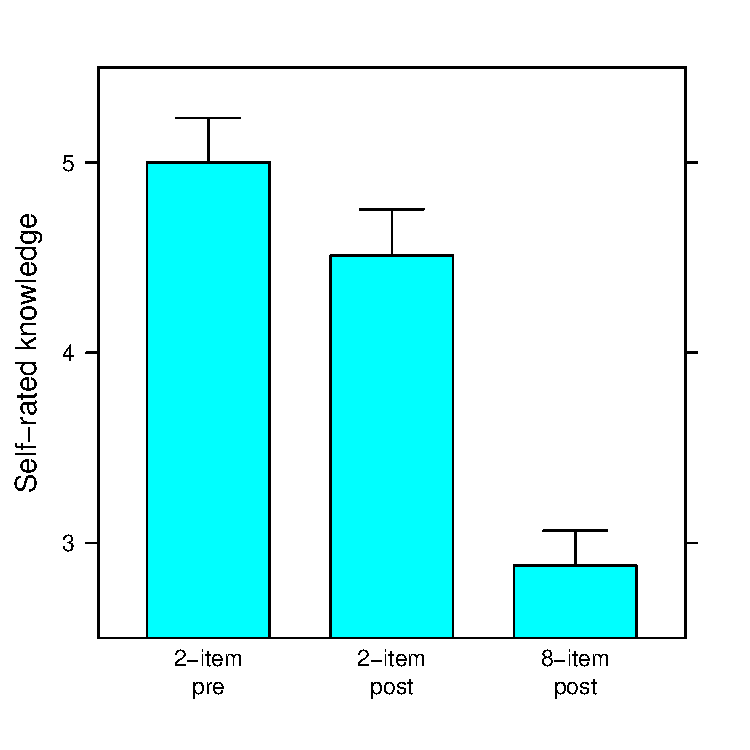
\includegraphics{evil-know.pdf}
    \caption{Self-rated knoweldge for individuals on pre- and post-tests. Again,
        pre-tests were only administered to individuals in the 2-item
        experimental variant.}
    \label{fig:evil-know}
\end{figure}

\subsection{Discussion}

In stark contrast to arguments that numeracy is polarizing
\parencite{kahan_polarizing_2012}, we have provided an existence proof that
appropriately selected scientific facts can have a profound effect in eroding
the existing beliefs of a population (i.e., “liberals” can be pushed in a more
“conservative” direction). In particular, we have demonstrated marked erosion of
self-confidence in one's own knowledge, as well as belief and concern regarding
anthropogenic climate change---even in our relatively liberal and
anthropogenic-climate-change-accepting sample of UC Berkeley undergraduates.
Such results were observed with as little as \emph{two} numbers.
% Still need to grab stuff from above
Consider the effect of Muller's writings prior to \textcite{rohde_new_2013}. A
prominent professor at our ostensibly liberal institution wrote extensively on
why we should doubt the veracity of climate change---including in the mainstream
media. We must assume that educated, liberal, GW-accepting individuals may be
easily swayed by a small dose of factual (but non-representative) numerical or
scientific information from such a source.

The primary point illustrated by this study is that individual's understandings
are demonstrably fragile. Even an intervention of a few minutes can massively
undercut individual's confidence in thier own knowledge, along with overall
belief and concern about global climate change. An additional point is that, as
noted by \textcite{kahan_polarizing_2012,mccright_politicization_2011}, surveyed
individuals were little-affected by self-guided educational efforts. Thus, one
might conclude that climate change accepters are unlikely to come into contact
with such numbers on their own.  However, there are concerted efforts to
distribute such numbers on the internet and elsewhere. A final point is that, as
shown above and as noted by \textcite{mccright_politicization_2011}, scientific
information might push individuals both towards scientific consensus, as well as
\emph{away} from it.  Thus, it seems wise to build a solid foundation of climate
change relevant knowledge in the American populace. 

It is clear that even relatively educated members of the public (e.g.,
undergraduates at a top-tier university) are highly susceptible to misleading,
cherry picked facts. Such facts are clearly known to organizations attempting to
undermine the overwhelming scientific consensus about climate change. Thus,
climate educators and communicators must counter the increasing sophistication
with which such organizations distribute misleading information.

\section*{Acknowledgements}

The work reported in this chapter has been previously published, in part, in
\textcite{clark_knowledge_inpress}.  All such material is re-used here with the
permission of my co-authors, the publishers, and the Graduate Division at the
University of California, Berkeley.


% These should get re-factored into proper chapters
% \graphicspath{{experimental-description/}}

\chapter{Summary and Experimental Aims}

In the background section, I laid out a number of general theoretical
orientations: the RTMD theory, the NDI program and multi-system analysis of
cognition. Our findings so far argue strongly for educational opportunities in
the domain of global climate change. In addition, we have been able to engage
individuals with both emotional and more conceptual aspects of psychological
processing in our educational interventions. I have not yet, however, provided
an analysis of NDI style climate interventions, or attempted to use the related
constructs available in the RTMD theory in the construction or enhancement of an
intervention. An NDI intervention has been developed and administered, and
analysis is underway.  Time permitting, the most proximal evolution and perhaps
nationalism constructs will be evaluated for their ability to influence
reasoning or learining about climate.

\begin{table}
\begin{tabular}{p{0.5\textwidth}p{0.5\textwidth}}
Result & Interpretation \\ \hline \hline
Objective scores of participant knowledge increase markedly from pre- to
post-test. & Even in relatively well-educated populations, individuals are
largely ignorant of the mechanism via which greenhouse gases increase global
mean temperature. However, this can be improved with a compact description. \\ \hline
The aggregate of climate change attitudes are improved from pre- to post-test. &
Continuing the above, individuals’ attitudes can also be influenced in a
positive way by a compact explanation. Teaching about the mechanism of global
warming yields shifts in attitudes! \\ \hline
Self-rated knowledge is positively correlated with objectively scored knowledge
when assessed prior to instruction. & Naïve individuals are at least somewhat
correct in their assessment of their knowledge of climate change relative to
their peers’ knowledge. \\ \hline
After instruction, the correlation between self-rated knowledge and objectively
scored knowledge reverses in the “Sandwich” group  & The sandwich intervention
appears to destabilize individuals’ metacognitive assessment of their own
knowledge. The more they learn, the less they think they know! (Note, post-test
correlations in the “No pre-test” group were not-quite-marginally positive.)
Note that the amount known initially is not predictive of self-rated knowledge,
or even objective post-test knowledge. \\ \hline 
Reported surprise is greater when individuals provide an explanation prior to
instruction. & As with results in the NDI paradigm, eliciting a participant’s
“best guess” may reduce post-hoc rationalization, thus increasing feelings of
surprise. This may be critical to obtaining the above-mentioned
“destabilization” of metacognition about one’s knowledge.  \\ \hline
Post-test self-rated knowledge is negatively correlated with surprise ratings in
the “No pre-test” group. & Again, if surprise is taken as a proxy for learning,
we find that such learning may even destabilize metacognition without the
enhancement provided by eliciting a participant’s best guess prior to
instruction.  \\ \hline
Global warming attitude ratings were not (significantly) correlated with
objective knowledge scores. &
It appears that self-assessment of knowledge--which is correlated with global
warming attitude ratings as well as objectively scored knowledge on various
tests--may be a critical link to obtaining attitude change via scientifically
grounded education. \\ \hline
\end{tabular}
\caption{Summary of results from mechanism study}
\label{table:mech-summary}
\end{table}

\begin{table}
\begin{tabular}{p{0.5\textwidth}p{0.5\textwidth}}
Result & Interpretation \\ \hline \hline

Estimation is more likely to improve than worsen after a delay of a day or more.
&
People will learn from a minimal intervention: providing participants with feedback after an estimation.
\\ \hline
Surprise is predictive of improved estimation. &
\multirow{3}{*}{\parbox{0.5\textwidth}{\vskip\baselineskip Surprise and metacognitive 
        assessments of memory may index separable cognitive processes. In
        particular, individuals may gain knowledge (in the form of an improved
        estimation) with no metacognitive awareness that they have done so.}} \\
\cline{1-1}
Metacognitive assessment of memory is predictive of improved estimation. & \\
\cline{1-1}
Surprise and metacognitive assessments of memory may index separable cognitive
processes. In particular, individuals may gain knowledge (in the form of an
improved estimation) with no metacognitive awareness that they have done so. &
\\ \hline
\end{tabular}
\caption{Summary of results from NDI memory study}
\label{table:two-summary}
\end{table}

In chapter~\ref{chap:ccc}, we observed (for now) isolated probabilistic
dependencies as shown in fig.~\ref{fig:causal-ccc}, and I have included a more complete
summary of results in table~\ref{table:mech-summary}. Chapter~\ref{chap:two}
found the probabilistic structure expressed in fig.~\ref{fig:causal-two}, and again I
have included a more complete summary in table~\ref{table:two-summary}. Recall
that in the NDI study, we are unable to attribute causality, while in the
mechanism study, due to the nature of the experimental manipulation, we can
assume the relationship between pre-existing knowledge and surprise is sound as
well as the mechanistic knowledge intervention's effect on climate change
acceptance. Below, I will lay out the results that need to be solidified from
the above research, as well as providing a few additional questions to be
answered by the thesis.

As summarized by figures~\ref{fig:causal-ccc} and \ref{fig:causal-two}, we have
managed to establish some predictive links between measurable variables. There
remain, however, various gaps which can be filled in by relatively obvious
variations on the experiments already done. In addition to the analysis of
existing data, I'm proposing one significant experiment per subsection below. In
addition, below I propose an additional 3 replication experiments using more
general populations. These experiments are intended to elucidate a set of links
such as those shown in fig.~\ref{causal3}.

\begin{figure}
\begin{center}
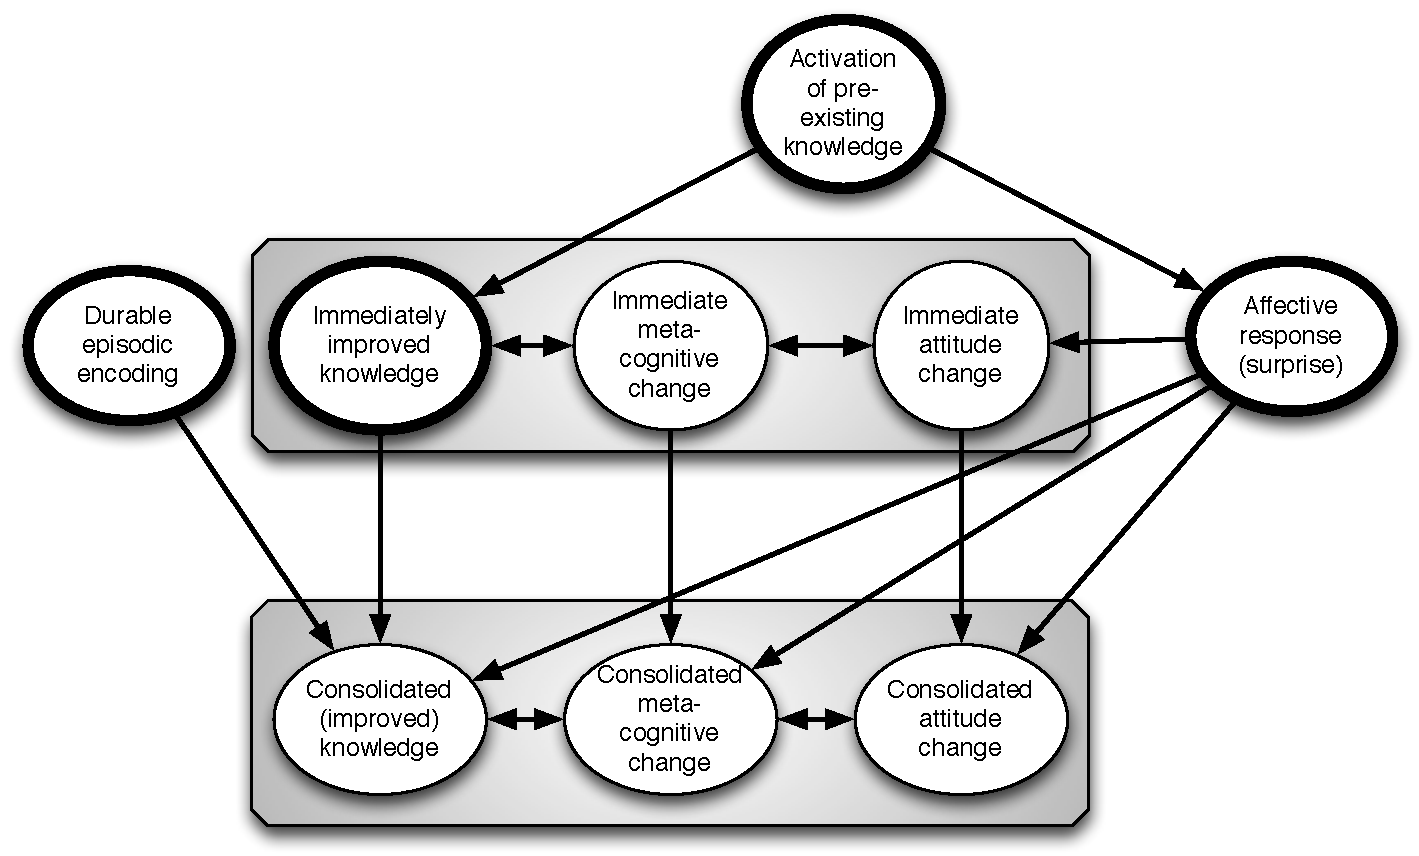
\includegraphics[width=\textwidth]{causal3.pdf}
\end{center}
\caption{A graphical model representing the potential relationships elucidated
    by the proposed experiments. Subjects internal representations are
    surrounded by grey boxes. Points of experimental manipulation are ringed by
    thick lines.}
\label{causal3}
\end{figure}

These experiments will draw on two forms of factual information: a
mechanistic description of the ``greenhouse effect'' and a number of lists of
numerical quantities that pertain to climate change and evolution. For the
purpose of the thesis, these items will be treated separately as opportunities
to elicit psychological processing and subsequent belief and attitude changes.

% In an ideal wold, this would probably get moved to the intro? Do this for
% thesis.
\section{A bit more theory}

One of the more established models of psychological processing of persuasive
messages is the Elaboration Likelihood Model \cite{petty_elaboration_1999}.
This model is (as might be expected) quite Elaborate, but for our current
purpose, it serves to note the following central observation in ELM research.
Specifically, changes in attitudes appear to be driven by at least two modes of
processing (or perhaps a spectrum between these modes) in which new information
may be deeply ``elaborated'' in a central process, or may alternatively be
incorporated peripherally via less effortful processing, such as heuristic or
emotional processing. Of critical concern to our educational goal, effortful
processing tends to yeild shifts that are durable and resistant to subsequent
counter-persuasion. Such persuasion might be crucial to the prevention of social
phenomena such as the gradual erosion of public acceptance of Climate Change
since the spike around the publication of ``An Inconvenient Truth'' 
\cite{leiserowitz_climate_2010}.

Yet another model of belief revision and behavioral change are the Theory of
Reasoned Action and the more elaborated Theory of Planned Behavior
\cite{montano_theory_2008}. In particular, the model posits that sets of
relatively concrete beliefs yeild more general attitudes (expressed as a latent
variable). These attitudes in turn guide individuals' behavior.  Here, I will
use a similar break-down of participants' mental representations, but introduce
an additional level of distinction. These distinctions may not be sharp in all
cases, but for the purposes of this experimental plan, they should be quite
clear. At a basic level, all of the experiments proposed herein operate at the
level of \emph{factual knowledge} (e.g., percentage decrease in ice in a
particular location). This knowledge in turn supports \emph{beliefs} regarding
the veracity of, e.g., anthropogenic climate change. Finally, I will refer to
\emph{attitudes} as consisting of an emotional link to some knowledge or belief.
Criticaly, the target of the emotional link needn't be accepted as true!

A recent model regarding the relationships and learning dynamics between
knowledge and emotional associations is the HOTCO model \cite{thagard_hot_2006}.
In the taxonomy I propose above, facts and beliefs could in principal exist
purely in the domain of ``cold cognition.'' In other words, one could hold ideas
about ice melt and even the reality of climate change solely on the basis of
evidence and inference.  Attitudes (as described above) are inherently emotional
(or ``hot''), however. As described by Thagard, the inferential links between
underlying facts and beliefs and their supported attitudes, such as concern
about climate change, will effect emotional responses to those supporting ideas.
So, for example, a person may have an attidue in which they worry about their
grandchildren's safety and health in the future. If we establish a coherent link
between climate change and this pre-esisting worry, that individual will then
come to worry about climate change. Emotional associations may similarly be
propigated to more basic factual knowledge, such as ice melt in a particular
location.

\section{Intentionally unanswered questions}

Prior to this writing, I have proposed a good number of potential experiments.
Due to pragmatic constraints, only a portion of these will be included in the
proposed thesis. For clarity, I include here a brief list of questions that I
plan to answer with work \emph{subsequent} to the thesis:

\begin{itemize}
    \item To what extent will reasoning and learning about "toy worlds" reflect
        reasoning and learning about real-world scenarioes in which individuals
        have a real, vested interest? Note - this is probably the most common
        question I get when discussing my work, so worth addressing even to get
        the negative result that I anticipate.
    \item What is the relative effectiveness of the various sorts of
        interventions employed here? For example, is suprising numerical
        information more or less effective at eliciting behavioral change than,
        say, appeals from authority or scientific exposition?
    \item To what extent can we characterize the nature of surprise and other
        affective responses at the physiological level? Can we observe emotional
        expressions using video capture? What about measures of respiration,
        heart rate, etc.?
\end{itemize}

\section{Central constructs and Aims}

Primary concern is behavioral change. For the purposes of these studies, we rely
primarily on measures of attitude (including expressed attitudes about planned /
anticipated behavior).

The primary measures are 

\begin{enumerate}
    \item Metacognition about one's knowledge (as it pertains to both the
        specific materials in a given study, as well as potentially the domain
        of climate change in general).
    \item Actual knowledge and change in knowledge (learning).
    \item Affective response to the materials being learned (surprise).
    \item Attitudes regarding climate change.
\end{enumerate}

In addition, a primary manipulation of interest is the elicitation (or not) of a
participant's prior knowledge. This has been shown to modulate surprise in some
of our initial data on climate change, and has been shown to modulate learning
in other studies mentioned above.

% Combine these "aims" with above

\subsection{Aim 1}

\textbf{Attempt to replicate existing effects across both mechanism and NDI based
    educational interventions, obtaining necessary statistical power where
    necessary}

% Determine the (large, obvious) interactions between (potentially)
%     concurrent psychological processes involved in the reading and understanding
%     of factual messages.

\begin{enumerate}
    \item At present, we have only observed reliable shifts in attitudes in UC
        Berkeley undergraduates. We have an existing dataset from UT
        Brownsville, but it is critical to establish the generality of our main
        findings by obtaining a broad sample.
    \item Of central interest from a psychological point of view, we have shown
        (via the mechanism manipulation) that increase in knowledge about
        climate change yeilds shifts in attitudes. However, we were unable to
        obtain a reliable relationship between attitudes and other experimental
        constructs. I expect that with more subjects, between subject
        variability in real and / or self-rated knowledge will significantly
        predict attitude change.
\end{enumerate}

%% This is largely similar to the above

% There are four separable (though not necessarily completely distinct) forms of
% psychological processing that will be measured: 
% 
% \begin{description}
%     \item[Durable episodic encoding] Participants will evaluate the extent of
%         their own learning. Specifically, subjects will be asked to make
%         remember / know style judgements on a numerical scale, as done in
%         experiment one. In addition, episodic encoding may be probed using
%         source detail memory. It should be noted that some degree of episodic
%         encoding is likely engaged for all items, but is simply not retained
%         (i.e., consolidated) in some cases. 
%     \item[Improved knowledge] Participants' actual improvements in their ability
%         to produce specific information. This will be measured either as
%         proximity to a correct numerical answer, or by using a rubric we've
%         developed to evaluate mechanistic descriptions.
%     \item[Interaction with pre-existing knowledge base] Some interaction with
%         participants' pre-existing knowledge is certain to occur. This can
%         manipulated, however, by asking participants to provide their own
%         estimates or explanations before providing them with the correct answer.
%         For the current set of experiments, we will not seek to suppress such
%         interactions.
%     \item[Affective response] Participants will be asked directly to evaluate
%         their reactions to presented items. In addition, for some experiments,
%         participants will be monitored directly using audio, video and
%         psysiological monitoring equipment (currently installed in Tolman 5503).
% \end{description}

\subsection{Aim 2}

\textbf{Extend the scope of data collected, in terms of temporal delay, number
    of participants and depth of survey / interview questions to establish
    further links between established theoretical constructs}

\begin{enumerate}
    \item Evaluate the longitudinal effects of our interventions on both
        knowledge and attitudes. To the extent possible, also probe for changes
        in behavior (or planned behavior).
    \item Refine our understanding of participant attitudes and responses. In
        particular, evaluate the meaning of subject responses on the
        ``surprise'' scale, and refine our assessment of climate change beliefs
        and attitudes.
\end{enumerate}

% Develop a predictive model for the durability and extent of belief and
%     attitude change from differing forms of psychological processing involved in
%     the reading and understanding of factual messages. As compared to aim 1,
%     here we intent to understand how participants generalize beyond the specific
%     information that they are given.}



% \graphicspath{{experimental-description/}}

\chapter{Experimental Plan}

\section{Completed and in-process experiemnts}

A summary of completed and in-process experiments is given in
Table~\ref{table:collected}. Further explanation is given, where warranted, in
the text below.

\begin{table}
\begin{tabular}{lp{0.25\textwidth}p{0.5\textwidth}}
Paradigm & Description & Status \\ 
\hline \hline
Mechanism study 
    & UC Berkeley class (2010) & Fully analyzed, chap.~\ref{chap:mechanism}. It
    remains to establish reliability in our coding scheme (see text). \\
    & UT Brownsville (2010) & Partially analyzed, no effect on climate attitudes \\
    & UT Brownsville (2011) & Data collected, but knowledge questions as yet
        uncoded, will be analyzed as with UC data \\

NDI study 
    & 2 UC Berkeley classes, 1 UT Brownsville (2011) & Data collected, currently
        being transcribed \\
\hline
\end{tabular}
\caption{Status of collected data-sets}
\label{table:collected}
\end{table}


\subsection{Mechanism Study}

While the methods are largely worked out for the mechanism study, there remains
a difficulty with coding the textual answers. If I am unable to develop an
efficient method for coding (i.e., automated, or otherwise train folks to code
more quickly), I will simply code a randomly chosen subsample of the data and
assume that the effects hold in the larger population (which will be used only
for attitude ratings, surprise, etc.) In any case, coding represents the only
remaining methodological piece of analyzing the mechanism data that hasn't been
finalized (although see section~\ref{sec:interviews} below for some
modifications to the common survey sections.

Currently, I have attempted a (relatively na\"ive) application of the na\"ive
Bayes algorithm to replicate codes (essentially a keyword-based approach which
ignores co-occurrences). This approach did not fare very well at all. I plan to
try similar methods to see if we are able to simply replicate the total scores.
In addition, Prof. Canny has recommended an exploration of "kernel based"
methods, in particular I plan to evaluate Latent Semantic Analysis and Latent
Dirichlet Analysis. In addition, Prof. Canny is offering a course in automated
text processing next semester.  This will be explored as time permits.

\subsection{NDI for climate change knowledge and attitudes}

A central limitation of the experiments in chapter~\ref{chap:two} was the lack
of a coherent message. Specifically, an intractable set of attitudes
would likely be affected by such a diverse collection of surprising facts,
including not only attitudes relevant to criminal justice, immigration, etc.,
but also to participants' sense of self-efficacy in terms of their numerical
reasoning!

The reasoning group has already developed an experiment-ready list of pro- and
anti-climate change acceptance numbers, and a similar list of evolution oriented
items is in process. These items will be used in experiments broadly similar to
that presented in chapter~\ref{chap:two}, but with the addition of an attitude
and belief survey as utilized in chapter~\ref{chap:mechanism}.

This experiment will allow us to observe the effects of a collection of facts
and consequent psychological processing on a related belief (e.g., reality of
climate change) and attitudes (e.g., worry about climate change, intention to
change behavior).

In particular, I am excited to see how surprise regarding numerical information
compares to surprise in the mechanism study.

\subsubsection{NDI with evolution numbers}

Time permitting, a set of evolution-relevant numbers will be provided to
participants in addition to climate items. The RTMD theory suggests that by
engaging this related attitude, we may alter cognition with respect to climate
change (in particular learning and attitudinal evaluation and change). This is
not, however, a central aim of the thesis.

\section{List of proposed experiments}

\begin{table}
\begin{tabular}{llp{0.5\textwidth}}
Paradigm & Description & Plan \\
\hline \hline
On-line surveys
    & Mechanism &  Analogous to experiment in chap.~\ref{chap:mechanism}. \\
    & Brief mechanism & If long-term attitude or conceptual change are observed
        using the full mechanism ``blurb,'' we may evaluate a shorter version,
        comprising only the shorter summaries from the blurb. \\
    & NDI (anti) & Directly analogous to the intervention used with Berkeley and
        Brownsville students this year. \\
    & NDI (pro) & Identical to the above, but with pro-climate change acceptance
        numbers. \\
    & NDI (evo) & An intervention utilizing a mixture of pro-climate and
        pro-global warming numbers. This may enhance the effect of the
        intervention due to something like general pro-science sentiment. \\

Clinical interviews 
    & Mechanism & Prior to aggressive nation-wide data collection,
    semi-structured interviews will be conducted both during and after the
    on-line version of the survey w/ RPP students. If warranted, this may be
    attempted with a laptop with the general public in public place, etc. \\
    & NDI & Similar to the above, focused on pro- and anti-climate change
        statistics \\
\hline
\end{tabular}
\caption{Proposed extensions of the above paradigms}
\label{table:proposed}
\end{table}

\subsection{On-line survey methodology}

Surveys will be delivered using qualtrics. Qualtrics provides for
straightforward subject tracking, which will allow us to administer follow-up
surveys with relative ease. CPHS approval has already been approved for these
approaches, including the ability to follow up with experimental participants
for a period of up to one year. This straightforward extension of our previous
interventions will allow us to answer one of the central questions in evaluating
their utility: ``Do our interventions have any long-term impact on knowledge
and/or attitudes?'' Both simpler regression-style approaches as well as full
blown growth models (a form of structural equation modelling) will be used to
evaluate these changes. Given practical concerns, while I plan to collect
longitudinal data at longer intervals, followups collected at one week
post-survey will be used to inform the thesis.

\subsection{Expansion and refinement of survey items}

In the proposed studies, I plan to continue the use versions of the instruments
described above regarding climate change and RTMD. Specifically, I'll continue
to use a mechanistic explanation of global warming, as well as an RTMD attitude
survey. In addition to these, the reasoning group continues to refine lists of
both pro- and anti-global warming and -evolution NDI style items. Given the
thesis' focus on psychological processing, variation in the stimulus set may
serve to lend credibility to the generalizability of any findings. However, care
will be taken to ensure that different sets of items are not provided to
fundamentally different subject populations. As a final point of comparison,
Joseph Williams (a collaborator) is planning to compare our mechanistic
explanation to other forms of argumentation from e.g. Al Gore's Climate Project
and the EPA website on climate change.

A basic issue regarding our ability to apply factor-based models is that we
should have three or more items per construct. This is a trivial problem, and I
plan to include additional items from Callie's study to bolster numbers for
under-represented constructs that are central to our experiment going forwards.
This will allow a more statistically sound evaluation of shifts in both the mean
values of constructs as well as the correlations between them.

\subsubsection{Undergraduate Interviews}
\label{sec:interviews}

A few constructs are not currently assessed in a highly accurate fashion. While
I had initially been considering applying physiological methods for capturing,
e.g., emotional response to survey items and the information presented, I am
instead taking a cue from psychophysics. To wit, individuals are profoundly more
sensitive to their own internal states than even the best physiological data
collection and analysis methods (notably, there may be aspects of experience
that are inaccessible to experience, and this may warrant followups with more
physiological measures). Thus, in order to gain greater purchase on participants
surprise, attitudes towards climate change, metacognition on their own knowledge
and learning, and so on. In particular, I plan to include more focused questions
regarding participants' responses to the material, including prompts to separate
what information was simply ``new'' as compared to ``convincing,''
``surprising'' or ``emotionally impactful.''

Permission for such interviews from CPHS is a pre-requesite to engaging in this
approach. While waiting for approval of this modification, I will conduct
surveys with RPP without interviews in order to pilot the on-line survey.

\subsection{Longer-term evaluation of learning and attitude change}

A surprising non-finding is that surprise is not terribly predictive of anything
in the mechanism experiment. This is likely because we have not allowed time for
the immediate effects of learning to dissipate. I expect that simply by
extending the time between the intervention and the post-test (at various lags
from a day to at least a few weeks), we will begin to see significant
predictions based on surprise. Specifically, I'd expect surprise (and other
affective responses) to predict better retainment or ``consolidation'' of the
factual knowledge, as well as more durable shifts in beliefs and attitudes. I
would expect enhancement of episodic encoding to have more of an effect towards
the factual end of subjects internal representations. Surprise, on the other
hand is likely have have broad effects.

\subsection{Subject selection}

Subject selection is a problem of central importance, given the inhomogeneity in
the population surrounding climate change and evolution acceptance. While, for
practical reasons, experiments will generally be run first at UC Berkeley, we
have already begun to collect data from remote locations. Specifically, we have
already obtained participants from a climate physics class in a southern Texas
university, many of whom reject climate change. In addition to recruiting
students from diverse universities, participants may be recruited from public
locations (Malls, DMVs), as well as from on-line. Based on the recommendation of
Prof. Canny and Joseph Williams, Facebook and Craig's list are the most likely
target for on-line participant recruitment, although other mechanisms will be
considered.

For the purposes of this thesis, I will seek to replicate the most central
results in a broader population as described above. In practical / contractual
terms, I expect to collect a total of 3 such experiments, distributed between
on-line and "real-life" populations.

Some of the potential effects we may observe are embedded within a large number
of variables, and may be relatively small (we cannot expect a lifetime of
climate change-related experience to be eradicated by a 10-minute
intervention!). Some require data-heavy techniques, like SEM to do regression on
latent variables. Thus, a primary experimental thrust will be to engage several
hundred participants in an on-line, somewhat expanded version of the experiment
described in chapter~\ref{chap:mechanism}.


% \graphicspath{{conclusion/}}

\chapter{Conclusion}
\label{chap:conclusion}

We have provided an evidential medley that effectively disconfirms the notion
that climate change-relevant knowledge and attitudes are locked in cognitive
stasis. Moreover, contrary to those who over-problematize a ``knowledge deficit''
(or ``information deficit'') approach to climate change communication, we see a
``wisdom deficit.'' Here (and in Ranney et al., 2012a) we have considerably
un-problematized it with the ``cognitive levers'' of these interventions. In
contrast, it is unlikely that offering either an ill-structured list of
uncompelling facts to an unprepared mind or thinly veiled rhetoric (cf. Lord,
Ross, \& Lepper, 1979) will notably alter beliefs or behaviors––especially about
the difficult topic of climate change. Rather, one must be sensitive to specific
(mis)understandings that may be relevant to a learner grappling with a domain.
Ultimately, we will likely need to engage virtually all people, assisting them
in connecting their long-term values to the long-term effects of their
behaviors.

In Study 2, we also showed, disturbingly, that one can readily erode climate
change acceptance with misleading, cherry-picked numbers. We can think of no
better protection against such ``evil'' interventions than to provide the context
necessary to recognize them for the clever misinformation that they are. Such
prophylactic interventions may represent promising targets for further research
and educational initiatives (cf. Lewandowsky et al., 2012).

We are currently studying ways of disseminating the information that we have
found to elicit worthwhile cognitive and belief changes.  For instance, we are
producing on-line instructional materials (e.g., videos) that can widely convey
both global warming’s mechanism and the statistics that reflect the scientific
consensus of climate change—so the public can join that consensus.

We have shown above that on-line survey interventions, brief curricula, and
classroom lessons can have a marked and persistent effect on knowledge,
understanding, beliefs, and attitudes about climate change. In spite of
arguments to the contrary, some simple cognitively-informed interventions might
be fundamental in building the resolve to tackle global climate change.


Summing up: going back to foundational thinkers in [American] education
(Dewey?). Is it "worth" educating individuals about climate change? In part, it
depends on who you are. If you are a science educator, I hardly needed to
complete this research to tell you that the answer is an emphatic YES! If you
are seeking to influence behavior or policy, however, it is a complex task. But
in contrast to the dominant view, it seems that science education might at least
push us in the right direction (even if it, alone, is not the most effective or
efficient route to conservation). But in the end, if it turns out that we are
indeed educable in a meaningful way, there is perhaps more value in conserving
the environment that sustains us than if we are mere automata to be shoved
around with propaganda!


% \bibliography{proposal,fixed}{}
% This is how biblatex does it
\printbibliography[heading=bibintoc]

\appendix

% \graphicspath{{appendices/kappa-extension/}}

% Note - pdf doesn't support extended characters in TOC
\chapter{Extension to Cohen's \texorpdfstring{$\kappa$}{kappa} for multiple scores}

Here, I'll describe exactly how I computed those $\kappa$'s for the mechanism
studies.

A note on using $\kappa$ in the text above: it seems completely admissable to
continue to use $\kappa$ for the measure described above, given it's similarity
in spirit to Cohen's original measure. This seems doubly admissable considering
that formal distributional considerations appear to be considered rarely, if
ever, in the psychological literature. Thus, any deviations in the specifics of
formal properties are unlikely to be a concern for the casual reader.

% \graphicspath{{graphical-models/}}

\chapter{Graphical Models}

There are numerous formalisms for representing informational relationships
between variables using shapes connected by lines or arrows (illustrated in
fig.~\ref{fig:bayes}). In this proposal, when I describe something as a
graphical model, I mean specifically that it is a directed Bayesian graphical
model (sometimes referred to as a ``Pearl net'' or a ``Bayes net''). Here I will use
``Bayes net'' for brevity.  There are two reasonable points of departure in
describing this formalism.

\begin{figure}
\begin{center}
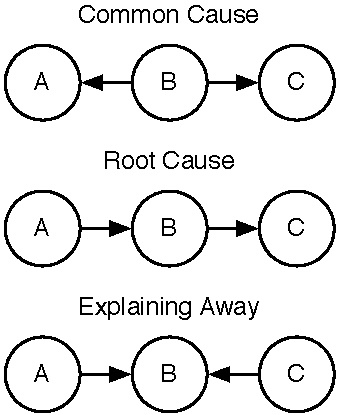
\includegraphics{bayes-nets.pdf}
\end{center}
\caption{A set of simple Bayes nets that illustrate the 3 topologies for a
    3-node, 2-link network.}
\label{fig:bayes}
\end{figure}

\section{Starting with SEM}

If you are familiar with the Structural Equation Modelling (SEM) formalism,
Bayes nets are quite similar, but differ in two
important ways. If you are \emph{not} familiar with SEM, please skip to the
following section. First, while SEM is a normal theory model (which allows for
relatively efficient estimation of parameters), each variable in a Bayes net may
have an arbitrary distribution. Sometimes pragmatic constraints are
placed upon these distributions, for example that they must come from the
exponential family. For their more descriptive useage in the proposal, such
constraints are unnecessary. A second difference is that the bidirectional arrows
signifying correlations in SEM are unavailable.

\section{Conditional independence}

Bayes nets are an easily human-interpretable representation of the conditional
dependencies (or lack thereof) between variables. In particular, there may be
(and usually is) a dependence between any two variables (nodes) in a Bayes net
if you are able to trace a path first up some set of arrows, and then down
another set. Thus, in fig.~\ref{fig:bayes}, A is independent of C only in the
``explaining away'' variation, where you can only reach C from A by going first
down, then up an arrow. Formally, a variable A is independent of B iff 
$p(A|B) = p(A)$.

Moreover, if the only way to get from A to C is via an intervening node B (or set
of intervening nodes), then A is conditionally independent of C given B. This is
the case in all three examples in fig.~\ref{fig:bayes}. Formally, 
$p(A|B,C) = p(A|B)$.

\chapter{Survey Items Used in Chapters \ref{chap:mechanism}, \ref{chap:prondi},
    \& \ref{chap:evilndi}}

\chapter{The 400 Words}
\label{chap:400}

\begin{center}
How does climate change (``global warming'') work?  The mechanism of the
greenhouse effect \\\relax
% Here and below, I could be using something like mchem, but \textsubscript is
% included with fixltx2e.
[Or: ``Why do some gases concern scientists---like carbon dioxide
(CO\textsubscript{2})---but not others, like oxygen?'']
\end{center}

Scientists tell us that human activities are changing Earth's atmosphere and
increasing Earth's average temperature. What causes these climate changes?

First, let's understand Earth's ``normal'' temperature: When Earth absorbs
sunlight, which is mostly visible light, it heats up. Like the sun, Earth emits
energy---but because it is cooler than the sun, Earth emits lower-energy infrared
wavelengths. Greenhouse gases in the atmosphere (methane, carbon dioxide, etc.)
let visible light pass through, but absorb infrared light––-causing the
atmosphere to heat up. The warmer atmosphere emits more infrared light, which
tends to be re-absorbed---perhaps many times---before the energy eventually
returns to space. The extra time this energy hangs around has helped keep Earth
warm enough to support life as we know it. (In contrast, the moon has no
atmosphere, and it is colder than Earth, on average.)

Since the industrial age began around the year 1750, atmospheric carbon dioxide
has increased by 40\% and methane has increased by 150\%. Such increases cause
\emph{extra} infrared light absorption, further heating Earth above its typical
temperature range (even as energy from the sun stays basically the same).  In
other words, energy that gets to Earth has an even harder time leaving it,
causing Earth's average temperature to increase---producing global climate
change. 

[In molecular detail, greenhouse gases absorb infrared light because their
molecules can vibrate to produce asymmetric distributions of electric charge,
which match the energy levels of various infrared wavelengths. In contrast,
non-greenhouse gases (such as oxygen and nitrogen––that is, O\textsubscript{2}
and N\textsubscript{2}) don't absorb infrared light, because they have symmetric
charge distributions even when vibrating.]

Summary: (a) Earth absorbs most of the sunlight it receives; (b) Earth then
emits the absorbed light's energy as infrared light; (c) greenhouse gases absorb
a lot of the infrared light before it can leave our atmosphere; (d) being
absorbed slows the rate at which energy escapes to space; and (e) the slower
passage of energy heats up the atmosphere, water, and ground. By increasing the
amount of greenhouse gases in the atmosphere, humans are increasing the
atmosphere's absorption of infrared light, thereby warming Earth and disrupting
global climate patterns.

\emph{Shorter summary}: Earth transforms sunlight's \underline{visible} light
energy into \underline{infrared} light energy, which leaves Earth slowly because
it is absorbed by greenhouse gases. When people produce greenhouse gases, energy
leaves Earth \underline{even more slowly}--\underline{raising} Earth's temperature.

\chapter{Mechanism items and coding scheme for responses}
\label{app:coding}

\section{Materials used by all coders}
\label{sec:materials}

Development of the coding scheme was a multi-step process. Initially, two
members of our group, Sarah Cohen and Roxana Farjadi, saught to identify
conceptions that occurred across multiple surveys. These conceptions were
assigned numerical codes, and these codes were arranged into general categories.
Following this, I developed a more complete progression, describing
relationships between the various categories, as well as grouping them into
“misconceptions,” “ignorance,” and “mechanistic description.” This allowed the
beginnings of a scoring rubric to be developed. We then iterated the process
with a larger group of coders to arrive at the final product reproduced below.
What follows is the full text of the coding packet developed by Ms. Cohen and
Ms. Farjadi, which also contains the text for the mechanism questions we
asked in our interventions. 

Note that \textcite{cohen_san_2012_f} also reports on a coding schema, though
that scheme exhibits differences with the one described here. Following this are
a diagram representing relationships between the codes. A section containing a
set of notes provided by Myles Crain are included in the next section. They
provides a set of criteria for chosing between notes, and was used by the final
set of coders. See chapter~\ref{chap:mechanism} for details.

% Note - there's actually a slightly more up-to-date version of this on google
% docs (edits by Baljeet and me)
\includepdf[pages=-,pagecommand={},landscape=true,scale=.85]%height=6.5in]
           {appendices/coding/codingpacket-blind-Oct26.pdf}

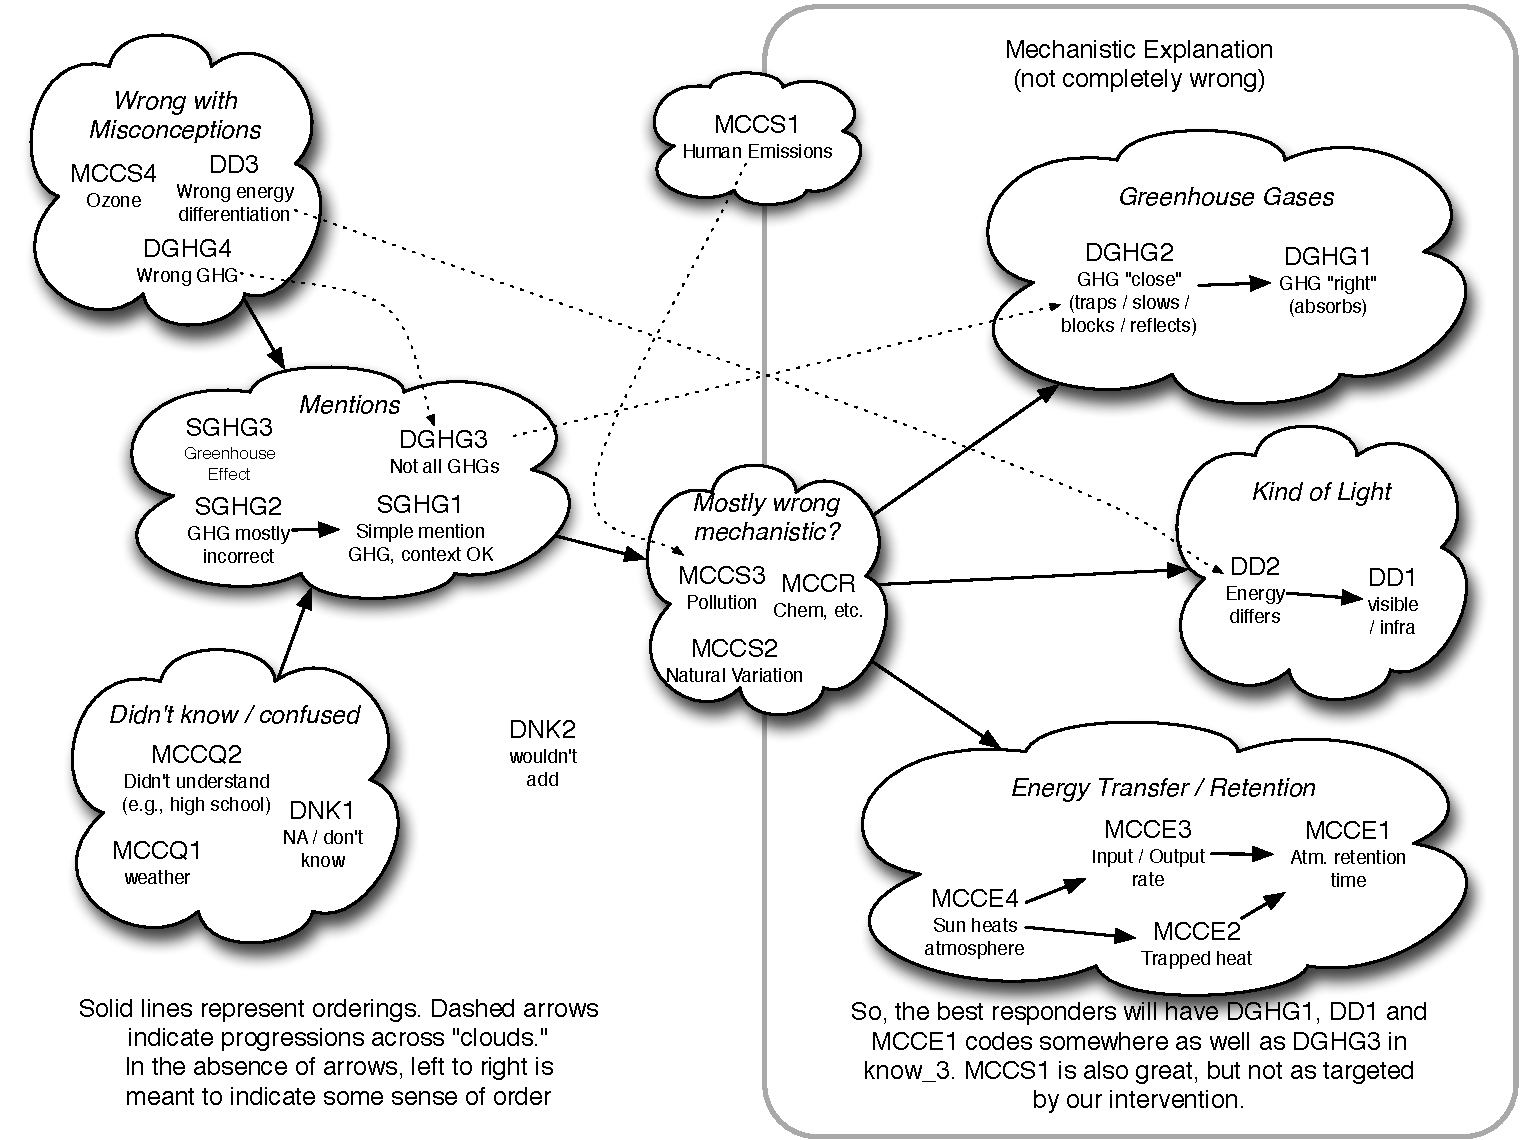
\includepdf[pages=1,pagecommand={},landscape=true,scale=.75]
           {appendices/coding/response-code-progression-letter-codes.pdf}

% Putting this in a landscape environment doesn’t do anything about
% the caption
% Here’s some code from tex.se:
% \begin{landscape} {\includepdf[pages={-},angle=90, offset=8mm 0mm,
% pagecommand={\begin{center}\textbf{~\Cref{fig:label} caption goes
% here.}\end{center}}, addtolist={ 1, caption for TOC goes here,
% tab:label}]{path/to/example.pdf} } \end{landscape}

% \begin{figure}[hp]
% 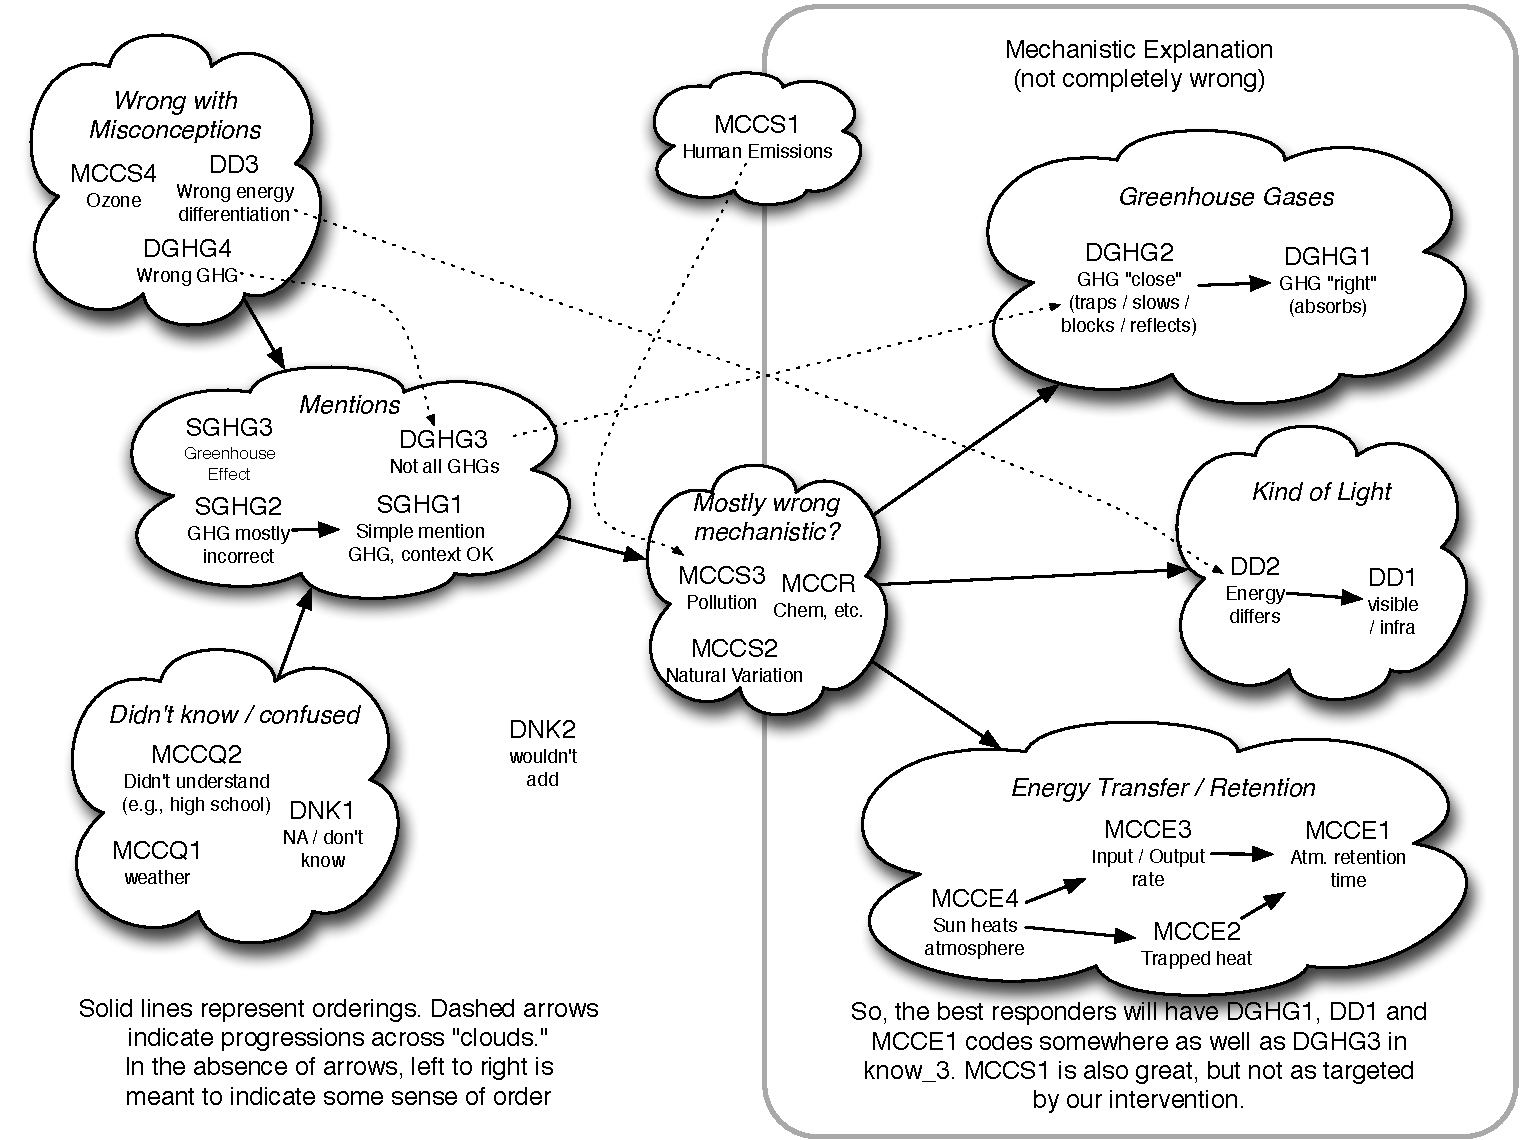
\includegraphics[height=6.5in,angle=90]{appendices/coding/response-code-progression-letter-codes.pdf}
% \caption{“Cloud” Diagram illustrating the relationship between codes}
% \end{figure}

\section{Notes on choosing codes}

This “crib sheet” was generated by Myles Crain to identify a single defining
characteristic and/or unique distinction within each code. Here are a few notes
on how it was used:

\begin{itemize}
\item The crib sheet is NOT self-contained. Its meant to jog memory
without having to constantly flip through the coding packet. The sheet
is only useful if you are generally familiar with the coding scheme
already.

\item Assigning a code should be defensible with explicit references to
the definitions and explanations of that code as provided in the
packet.

\item I've separated DGHG3 from the other DGHG codes intentionally (that
is, DGHG3 coming after DGHG4 is NOT a typo).

\item SGHG codes are only supposed to be used in the complete absence of a
definition of GHGs. The SGHG category is primarily useful in coding
for whether an explanation of climate change includes explicit
reference to GHGs.

\item Use MCCE codes to identify how a participant refers to energy within
an explanation of climate change.

\item Enquoted things are things that must appear in a response in order
to apply the code (except when there are other options--for example,
SGHG1 requires using the phrase "GHG" *or* citing specific examples of
GHGs).
\end{itemize}
Following is the “crib sheet” itself:

\begin{description}
\item[DD1] visible incoming \& infrared outgoing
\item[DD2] asymmetry/difference reference
\item[DD3] wrong, no asymmetry/difference
\vspace{7pt}
\item[DGHG1] GHGs "absorb" energy
\item[DGHG2] part correct, no "absorb"
\item[DGHG4] wrong
\item[DGHG3] "not all", cite >1
\vspace{7pt}
\item[SGHG1] "GHG"/e.g., mostly accurate
\item[SGHG2] "GHG"/e.g., mostly wrong
\item[SGHG3] "greenhouse effect"
\vspace{7pt}
\item[MCCE1] more gas/heat than before
\item[MCCE2] heat/energy "trapped"
\item[MCCE3] different input/output rates/amounts
\item[MCCE4] sun's radiation heats atmosphere
\vspace{7pt}
\item[MCCS1] humans/tech/fossil fuels
\item[MCCS2] natural variation
\item[MCCS3] pollution
\item[MCCS4] O3 layer
\vspace{7pt}
\item[MCCR] chemical/molecular exclusively
\item[MCCQ1] weather, confusion
\item[MCCQ2] irrelevant
\vspace{7pt}
\item[DNK1] "don't know", n/a
\item[DNK2] nothing added
\end{description}

\section{Assigning scores to coded responses}

Detail here the procedure for assigning scores to codes. Perhaps even include
the R or python code?

% \chapter{Format of final NDI intervention}
\label{app:format-ndi}

Below is an example format for an NDI-style estimation intervention.
Interventions consisted of 2-8 such estimations, and did not always include all
elements (see individual sections for details). Note also that I have not
adjusted the formatting to avoid \LaTeX\ defaults, such as indentation. 
\hrule
Global surface temperatures have been recorded since 1850. According to the IPCC
Fourth Assessment Report, released in 2007, how many of the years between
1995-2006 (a 12 year period) are one of the hottest 12 years of recorded global
temperature? My estimate is a…

number of years (out of 12)

The number I estimate is (whole numbers only):

How low and how high would that number have to be to surprise you?
Lower than: 
Higher than:

Approximately how confident are you that the actual value falls in the range
between the low and high numbers above? (Note that a confidence below 50 would
imply you think it is more likely that the number is outside your range!)

\underline{\hspace{3cm}} Percent Confidence (selected with slider ranging from
50–100)

 
On the previous page you estimated the following value:  Global surface
temperatures have been recorded since 1850. According to the 2007 report from
the Intergovernmental Panel on Climate Change, how many of the years between
1995-2006 (a 12 year period) are one of the hottest 12 years recorded?

The true value is: 11 years  Please note how this compares to the estimate you
gave: [estimate is inserted here] (number of years)

Did you find this number surprising?

Not Surprising at All 1, 2, 3, 4, Somewhat Surprising 5, 6, 7, 8, Extremely
Surprising 9

Briefly, what specifically did you find surprising (if anything)?

Were you surprised or embarrassed at your own lack of knowledge?

Not Surprised or Embarrassed at All 1, 2, 3, 4, Somewhat Surprised or
Embarrassed 5, 6, 7, 8, Extremely Surprised or Embarrassed 9

How novel or familiar is this information to you?

I've seen nothing like this 1, 2, 3, 4, I've seen similar information 5, 6, 7,
8, I've seen this exact informaiton 9 

Please describe anything you'd forgotten prior to reading the value above, but
now you remember (if anything):

Please describe any other thoughts or memories triggered by the above, including
if you have any points of disagreement or objection (if anything):

% \chapter{Numerical Information used in Chapter \ref{chap:prondi}}
\label{app:numbers}

Note that we do not report the specific information used in \ref{chap:evilndi},
as we have little desire to contribute to the precision of the already
formidable propaganda campaign arrayed against climate change acceptance.

The below is not formatted well for \hologo{LaTeX}.


Global surface temperatures have been recorded since 1850. According to the 2007 report from the Intergovernmental Panel on Climate Change, how many of the years between 1995-2006 (a 12 year period) are one of the hottest 12 years recorded?
"\# of years"
11 years

What is the change in the atmospheric levels of methane (a greenhouse gas) since 1750?
"\% increase" or "\% decrease"
151\% increase

What is the change in percentage of the world's ocean ice cover since the 1960s?
"\% increase" or "\% decrease"
40\% decrease

According to observation data collected at Mauna Loa Observatory in Hawaii, what is the percent change in atmospheric CO2 levels from 1959 (when observation began) to 2009?
"\% increase" or "\% decrease"
22.6\% increase

A 2010 article examines the 908 active researchers with at least 20 climate publications on Google Scholar. What percentage of them have stated that it is “very likely” that human-caused emissions are responsible for “most” of the “unequivocal” warming of the Earth in the second half of the 20th century?
"\% of researchers"
97.5\%

In 1850 there were approximately 150 glaciers present in Glacier National Park. How many are present today?
"\# of glaciers"
25 glaciers

From 1850 to 2004, what is the percent change of volume of glaciers in the European Alps?
"\% increase" or "\% decrease"
50\% decrease

(Note - actually reported 6.4 feet on all but final CCO studies - will be final
2 once I run Michael's proposed changes)
According to a study published in Geophysical Research Letters, by how much has the average sea level changed from 1870 to 2004?
"feet increase" or "feet decrease"
0.640 feet



\end{document}
